% https://www.smu.ca/academics/archives/honours-thesis.html#d.en.48587
% https://www.smu.ca/webfiles/th027_honours_format_procedures.pdf




\documentclass[11pt]{report}
\author{Justin Gray}
\title{The Practical Efficiency of Regular Expression Membership Algorithms}

% set the margins to 1"
\usepackage{geometry}
\geometry{margin=1in}

% multiple columns (ie, figure comparisons)
\usepackage{multicol}
\setlength{\columnsep}{1cm}

% double space everything by default
\usepackage{setspace}
\doublespacing
\setlength{\parskip}{12pt}

% code segments
\usepackage{listings}
\lstset{
  numbers=left, 
  frame=single, 
  basicstyle=\singlespacing\ttfamily, 
  mathescape=true
}
\renewcommand{\lstlistingname}{Algorithm}
\renewcommand{\lstlistlistingname}{List of \lstlistingname s}

% math stuff
\usepackage{amsfonts} % mathbb{N} etc
\usepackage{amsmath}
\usepackage{mathtools}

% graphs
\usepackage{tikz-qtree}
\usetikzlibrary{automata}
\usetikzlibrary{fit}

% subfigure environment
\usepackage{subcaption}
\captionsetup{compatibility=false}

% bibliography
\usepackage[
    backend=bibtex, 
    sorting=none, 
    citestyle=numeric-comp,
    maxbibnames=100
  ]{biblatex}
\bibliography{refs}

% misc imports
\usepackage[                  % to bring \todo into scope
    backgroundcolor=lightgray, 
    textsize=tiny
  ]{todonotes}
\usepackage{indentfirst}      % to indent the first paragraph after a chapter/section
\usepackage{float}            % so figures can be positioned [H]ere
\usepackage{hyperref}         % clickable citations and sections
\usepackage[utf8]{inputenc}   % allows 2-byte characters like ï

\begin{document}

  \begin{titlepage}
  \begin{center}
    {\Large The Practical Efficiency of Regular Expression\\
    Membership Algorithms}
    
    \vspace{1cm}
    
    By Justin Gray

    \vspace{1cm}
    
    \begin{singlespace}
    	A Thesis Submitted to \\ 
    	Saint Mary's University, Halifax, Nova Scotia \\
    	in Partial Fulfillment of the Requirements for \\
      the Degree of Bachelor of Science, Honours Computing Science.
    \end{singlespace}
    
    \vspace{1cm}
    
    April 2022, Halifax, Nova Scotia
    
    \vspace{1cm}
    
    Copyright Justin Gray, 2022
    
    \vfill
    
    {\flushright\singlespacing
      \begin{tabular}{ r l }
      	Approved: & Dr. Stavros Konstantinidis \\
      	\empty & Professor, Supervisor \\
      	\empty & \empty \\
      	\empty & \empty \\
      	\empty & \empty \\
      	
      	Approved: & Dr. Porter Scobey \\
      	\empty & Associate Professor, Reader \\
      	\empty & \empty \\
      	\empty & \empty \\
      	\empty & \empty \\
      	
      	Date: & \today
      \end{tabular}\\    
    }    
  \end{center}
\end{titlepage}
  \begin{center}
  {\Large The Practical Efficiency of Regular Expression\\
  Membership Algorithms}
  
  By Justin Gray
  
  \vspace{1cm}
  
  {\bf Abstract}\\
\end{center}

\begin{onehalfspace}
  Regular expressions encode text patterns and define languages of symbolic words. The membership problem decides if a given word is an element of the language described by a given regular expression. This problem has various well-studied algorithms, but current research only shows asymptotic complexity and performance with respect to samples of randomly generated regular expressions. Our research aims to answer how the algorithms perform when using practical regular expressions used in the real-world on a representative test set of words. A set of compatible regular expressions have been collected from public GitHub repositories. Each compatible expression (i.e., no backreferences or improper formatting) is then converted into an equivalent unambiguous mathematical representation. For each distinct expression, we have tested Thompson, Glushkov, position, follow, and partial derivative NFA constructions, as well as partial derivatives and exponential backtracking directly on the regular expression tree. These algorithms have been implemented into a modified version of the Python’s FAdo library and include UNIX-inspired extensions such as character classes, the wild dot, and UTF-8 support. We find that efficiently constructing a small NFA is the best approach to this problem; using follow and PDDAG algorithms are experimentally shown as the best.
\end{onehalfspace}
  
\vfill
  
{\flushright \today \\}
  
  {\singlespacing \tableofcontents}

  \chapter{Introduction}
  \label{ch:Introduction}
  The most fundamental question with respect to regular expressions is asking if a given input word is accepted by a given regular expression. This is called the membership problem, and it returns a simple boolean answer. Most practical solutions to this problem have significantly deviated from their theoretical roots, by extending regular expressions to accept non-regular languages, as well as using exponential backtracking approaches rather than current developments in the theoretical field. As the theory has evolved, publications have been accompanied by asymptotic analyses. But to our knowledge, a real-world practical study of these improvements has not been conducted.

This research will test various algorithms for solving the membership problem on practical regular expressions used by developers. There are two distinct classes of algorithms: backtracking and partial derivatives can be computed directly on a regular expression, and automata solutions built using Thompson, Glushkov, position, follow, and partial derivative constructions. Which algorithms applied to the membership problem are the fastest with respect to practical regular expressions? How does the exponential backtracking algorithm compare with its theoretical counterparts? If you were writing a modern regular expression library today, which algorithms should be included for membership evaluation?

We begin in Chapter \ref{ch:Background} with a basic overview of essential regular expression related topics. Chapter \ref{ch:Literature Review} goes beyond widely understood topics and explores techniques and constructions useful for the rest of the project. In Chapter \ref{ch:Programming Tools} useful libraries and programming tools are briefly explained. The methods and implementation details are given in Chapter \ref{ch:Methodology}. Finally, in Chapters \ref{ch:Results} and \ref{ch:Conclusions} we discuss the results of the experiments and provide some directions for further research.
  
  \chapter{Background}
  \label{ch:Background}
  To ensure anyone with a moderate mathematical background can understand the contents of this paper, relevant introductory concepts are explained in this chapter. It is recommended that special attention be given to Sections \ref{sec:Regular Expressions} - \ref{sec:Finite Automata}, as the concepts therein will be critical throughout the paper. Advanced readers who are familiar with formal language theory should at least glance through these highlighted sections to understand the important difference between a \emph{programmer's regular expression} and a \emph{mathematical regular expression}, as well as our state notation for NFA constructions.





\section{Formal Languages}
\label{sec:Formal Languages}
Formal languages study \emph{words} created by \emph{alphabets} in \emph{languages}. Many real-world problems can be encoded in terms of languages: is a given word an element of a specified language, or how large is the defined language?
\begin{enumerate}
  \item {\bf Alphabet:} a non-empty set of symbols (characters) typically denoted by $\Sigma$. Some alphabets are used frequently enough to be given a name: the binary alphabet is represented by $\Sigma_2 = \{0, 1\}$.
  \item {\bf Word:} an ordered sequence of concatenated (joined) symbols from an alphabet. For example, $0110$ and $10011$ are words over the binary alphabet. When no symbols are chosen we refer to the empty word as $\epsilon$. The empty word has the special concatenation property: $w \equiv w\epsilon \equiv \epsilon w$.
  \item {\bf Language:} a set of words on an alphabet. The language $\Sigma^*$ represents the set of all possible words of any length on a given alphabet. Every language is a subset of $\Sigma^*$.
\end{enumerate}
Since languages are simply sets, the following important set operations on languages $K$ and $L$ exist:
\begin{enumerate}
  \item Union: $K \cup L = \{w : w \in K $ or $ w \in L\}$
  \item Concatenation: $K \odot L \equiv KL = \{uv : u \in K, v \in L\}$
  \item Power: $K^n = \{u_1 u_2 ... u_n : u_i \in K\}$. Note that $K^0 = \{\epsilon\}$
  \item Kleene Star: $K^* = K^0 \cup K^1 \cup K^2 \cup K^3 \cup K^4 ...$
  \item Difference: $K \backslash L = \{w : w \in K, w \notin L\}$
  \item Complement: $K^c = \Sigma^* \backslash K$
\end{enumerate}





\section{Regular Expressions}
\label{sec:Regular Expressions}
Non-trivial language problems involve large languages. It becomes unmanageable to explicitly enumerate every word in the language, and impossible for infinitely large languages. Regular expressions aim to solve this problem by encoding many languages in a relatively small sequence of alphabet symbols and meta-character operations. We distinguish two types of regular expressions in this paper: mathematical regular expressions and programmer's regular expressions. In each case, the function $L(\alpha)$ represents the language encoded by the regular expression $\alpha$. A regular expression $\alpha$ \emph{matches} or \emph{accepts} a word $w$ if and only if $w \in L(\alpha)$.

Mathematical regular expressions represent the most simple specification. Any language that can be encoded using a mathematical regular expression is classified as a \emph{regular language}. These expressions are defined inductively over the alphabet $\Sigma \cup \{(, ), *, +, \oslash\}$. 

{\bf Definition of Mathematical Regular Expressions}
\begin{enumerate}
  \item Atomic regular expressions $\oslash$ and $\sigma \in \Sigma$ such that $L(\oslash) = \emptyset = \{\}$ and $L(\sigma) = \{\sigma\}$
  \item Composite regular expressions from given regular expressions $\alpha$ and $\beta$:
    \begin{enumerate}
      \item Disjunction: $(\alpha + \beta)$ accepts $L(\alpha) \cup L(\beta)$
      \item Kleene Star: $\alpha^*$ accepts $L(\alpha)^*$
      \item Concatenation: $(\alpha \odot \beta) \equiv (\alpha \beta)$ accepts $L(\alpha) L(\beta)$ \\
            If $\alpha$ and/or $\beta$ are $\oslash$, then it accepts $\emptyset$
    \end{enumerate}
\end{enumerate}
In this thesis we extend this definition with compatible structures that maintain regularity:

\begin{enumerate}
  \item Option: $\alpha?$ accepts $L(\alpha) \cup \{\epsilon\}$
  \item Empty Word: $\epsilon$ accepts $\{\epsilon\}$
  \item Wild Dot: $.$ accepts $\Sigma$
  \item Character Classes: a non-empty sequence of symbols $\sigma$ and inclusive symbol ranges $\sigma_1-\sigma_2$ ($\sigma_1 \leq \sigma_2$) enclosed within [ ] for positive matches or [$^\wedge$ ] when looking for any symbol not contained within the character class. Some examples below:
    \subitem $L([abc]) = \{a, b, c\}$ 
    \subitem $L([^\wedge abc]) = \Sigma \backslash \{a, b, c\}$
    \subitem $L([0-9abcx-z]) = \{0, 1, ..., 9, a, b, c, x, y, z\}$
\end{enumerate}

Mathematical regular expressions form regular expression trees. The tree length of a regular expression is defined as the number of nodes in its tree. Figure \ref{fig:regexp_tree} shows a regular expression tree of tree length 9 using most of the features noted above: concatenation (explicit $\odot$), disjunction (+), Kleene star (*), simple atoms (a, b), wild dot (.), and the character class ($[012c-z]$).

\begin{figure}[H]
  \centering
  \Tree 
  [
    .$\odot$ 
    [
      .$+$ 
      a 
      [
        .$^*$ 
        b 
      ]
    ]
    [
      .$\odot$ 
      [
        .? 
        $.$ 
      ]
      $[012c-z]$ 
    ]
  ]
  \caption{A regular expression tree for the mathematical regular expression $((a + b^*) (.? [012c-z]))$}
  \label{fig:regexp_tree}
\end{figure}

{\bf Programmer's Regular Expressions}

Programmer's regular expressions are used in practical software applications \cite{formal-regexps}. Their typical implementations further extend the definition of mathematical regular expressions from above. Because of certain non-regular operations such as backreferences, only a subset of programmer's regular expressions can be converted into mathematical regular expressions. And from a theoretical point of view, programmer's regular expressions do not define regular languages, but instead a higher subclass of recursively enumerable languages. Converting programmer's regular expressions into mathematical regular expressions is explored in Section \ref{sec:Sampling Practical Regular Expressions}. Among other features, programmer's regular expressions:

\begin{enumerate}
  \item Change the disjunction operator from plus ($+$) to pipe ($|$).
  \item Remove the explicit representation of the empty word in favour of using the option operation.
  \item Allow for implicit operations defined by precedence rules.
  \item Add anchors: typical implementations of programmer's regular expressions consider a given word to be in the language if any substring of the word is in the language. This substring rule can be disabled by anchoring the expression. Placing a $^\wedge$ at the start of the regular expression asserts the match begins at the start of the string, and placing a $\$$ at the end ensures nothing can be matched afterward. In Section \ref{subsec:Partial Matching} we define a mapping from anchored expressions into mathematical expressions.
  \item Add ranged repetitions: the syntax $r\{n,m\}$ encodes the power operation on $r$, between $n$ to $m$ times (inclusive). If $n$ is missing it defaults to 0, and if $m$ is missing it defaults to $\infty$. Section \ref{subsec:Converting into FAdo Compatible Syntax} shows how a ranged repetition can be equivalently expressed using concatenations, disjunctions, and $\epsilon$'s.
  \item Add backreferences: this non-regular language operation allows matching the same substring multiple times. Regular expressions cannot represent the language $\{ww : w \in \Sigma^*\}$, but we can using the backreferencing expression $^\wedge (.^*)\backslash 1 \$$. Unless the initial match encodes a finite sub-language, we are unable to convert any expression with a backreference into the above mathematical definition. In general this is not the case, and we therefore do not consider any programmer's regular expression containing backreferences.
\end{enumerate}

A regular expression $r$ matches/accepts a word $w$ if and only if $w \in L(r)$. Determining the practical efficiency of this membership problem is the focus of this research, and has several different approaches. Throughout this paper, mathematical regular expressions may not be fully parenthesized and will instead rely on implicit precedence rules to improve conciseness. These precedence rules are given in descending order: star, optional, concatenation, and disjunction. Mathematical regular expressions may briefly contain anchors before being removed; in such a case the anchors are treated as $\epsilon$.

Typically regular expressions are seen as presented above, where binary operators like concatenation and disjunction are placed in the middle of two sub-expressions, or where the star and optional are placed immediately after a sub-expression. However, it can occasionally be useful to use an alternative string syntax called reverse polish notation (RPN) where operators are never implicit and always come before their sub-expressions. Given regular expressions $\alpha, \beta$ in the appropriate form, the following equivalencies exist:

\begin{center}
  \begin{tabular}{c|c|c}
    Infix             & Operation     & RPN \\
    \hline
    $(\alpha \beta)$  & Concatenation & $\odot \alpha \beta$ \\
    $(\alpha + \beta)$ & Disjunction  & $+ \alpha \beta$ \\
    $\alpha^*$        & Star          & $^* \alpha$ \\
    $\alpha?$         & Optional      & $? \alpha$ \\
    $\sigma$          & Atom          & $\sigma$ \\
    $\epsilon$        & Empty word    & $\epsilon$
  \end{tabular}
\end{center}

The RPN syntax is equivalent to the typically-used infix syntax, but hurts human readability in favour of removing parentheses and being more compact. For example, the mathematical regular expression $(a + (b^*)) \odot ((.?) \odot [012c-z])$ from Figure \ref{fig:regexp_tree} becomes $\odot + a ^*b \odot ? . [012c-z]$ when expressed using RPN.






\section{Derivatives}
\label{sec:Derivatives}
Derivatives can be applied both to languages and regular expressions. The high-level idea is to remove the first symbol from each word and see what remains. The derivative of a language $L$ relative to a symbol $a$ is the language defined as $a^{-1} L = \{y : ay \in L\}$. An arbitrary word $w = a_1a_2...a_n$ is an element of $L$ if and only if $\epsilon \in a_n^{-1}...a_2^{-1}a_1^{-1} L$. That is, removing the first letter $a_1$ from the words of $L$, then the first letter $a_2$ from the resulting words and so on will result in a language. If this language contains the empty word $\epsilon$, then $w = a_1a_2...a_n$ is in $L$. Derivatives for regular expressions are defined inductively \cite{brzozowski1964}. 

\begin{enumerate}
  \item $D_\sigma(\alpha \beta) = \begin{cases}
      D_\sigma(\alpha) \beta,              & \epsilon \notin L(\alpha) \\
      D_\sigma(\alpha) \beta + D_\sigma(\beta), & \epsilon \in L(\alpha)
    \end{cases}$
  \item $D_\sigma(\alpha + \beta) = D_\sigma(\alpha) + D_\sigma(\beta)$
  \item $D_\sigma(\alpha^*) = D_\sigma(\alpha) \alpha^*$
  \item $D_\sigma(\sigma) = D_\sigma(.) = D_\sigma([...\sigma...]) = \epsilon$
  \item $D_\sigma(a) = D_\sigma(\oslash) = \oslash$, for $a \neq \sigma$
\end{enumerate}
The derivative of a regular expression is a regular expression. For example,
\begin{center}
  $D_a((a + b*) (a (ba)^*)) = ((a (ba)^*) + (ba)^*)$  
\end{center}
An arbitrary word $w = a_1a_2...a_n$ is accepted by regular expression $r$ if and only if $\epsilon \in L(D_{a_n}...D_{a_2}D_{a_1}(r))$. Although derivatives can solve membership of infinite languages, the returned expressions suffer from exponential growth \cite{Antimirov}.

Mirkin and Antimirov introduced partial derivatives as an improvement to Brzozowski's word derivatives \cite{Antimirov, mirkin66}. Partial derivatives use sets of regular expressions instead of a single regular expression to maintain the derivative's value.
\begin{enumerate}
  \item $\delta_\sigma(\alpha \beta) = \begin{cases}
      \delta_\sigma(\alpha) \{\beta\},                        & \epsilon \notin L(\alpha) \\
      \delta_\sigma(\alpha) \{\beta \} \cup \delta_\sigma(\beta), & \epsilon \in L(\alpha)
    \end{cases}$
  \item $\delta_\sigma(\alpha + \beta) = \delta_\sigma(\alpha) \cup \delta_\sigma(\beta)$
  \item $\delta_\sigma(\alpha^*) = \delta_\sigma(\alpha) \{\alpha^*\}$
  \item $\delta_\sigma(\sigma) = \delta_\sigma(.) = \delta_\sigma([...\sigma...]) = \{\epsilon\}$
  \item $\delta_\sigma(a) = \delta_\sigma(\oslash) = \emptyset$, for $a \neq \sigma$
\end{enumerate}

The derivative example is redone using partial derivative rules, and we get a set of regular expressions rather than a single regular expression:
\begin{center}
  $\delta_a((a + b*) (a (ba)^*)) = \{a (ba)^*, \{(ba)^*\}$  
\end{center}

Let the $pd(r)$ function represent the set of all regular expressions derivable by repeatedly applying the partial derivative algorithm on every element with respect to each character of the alphabet $\Sigma$. This set of regular expressions can be no larger than the alphabet length of the regular expression. That is, $|pd(r)| \leq |r|_\Sigma$ \cite{Antimirov}. This theorem makes testing if a regular expression $r$ accepts $w = a_1a_2...a_n$ easy and efficient:

\begin{lstlisting}[label=alg:pd-match, caption={Partial derivative membership}]
Algorithm PD Match($r$, $w$):
    current := $\{r\}$
    for each $a_i$ in $w$:
        next := $\emptyset$
        for each $\beta$ in current:
            next := next $\cup$ $\delta_{a_i}(\beta)$
        current = next
    for each $\beta$ in current:
        if $\epsilon \in L(\beta)$ return Yes
    return No
\end{lstlisting}

As identified by Antimirov, one of the most expensive parts of this algorithm is testing equality of regular expressions to maintain sets of unique elements, current and next. Significantly reducing or entirely eliminating this cost without using automata remains an open problem, but can be mitigated by assigning each regular expression subtree with a directly comparable string or number.





\section{Finite Automata}
\label{sec:Finite Automata}
A finite automaton is an alternative way to express a regular language. Formally, a finite automaton is a 5-tuple $(Q, \Sigma, q_0, \delta, F)$. Where $Q$ is a set of states (labelled graph nodes), $\Sigma$ is the alphabet of the language, $q_0$ is the initial state, $\delta \subseteq (Q, \Sigma, Q)$ is the transition function of atomic structures between states (directed labelled edges), and $F$ is the set of final states. The transition function $\delta$ maps a state $p$ and a symbol $\sigma$ to the set $\delta(p, \sigma)$ of possible next states. We also view $\delta$ as the set of transitions (edges); that is, $(p, \sigma, q) \in \delta$ means that $q \in \delta(p, \sigma)$. For an automaton $A$, the language $L(A)$ consists of all input words leading from the state $q_0$ to any final state in $F$ through zero or more transitions defined by $\delta$. In general the transition function is non-deterministic; meaning there can be multiple successors of a state given a single label. Deterministic transition functions also exist, but could require an exponentially larger automaton than their non-deterministic counterparts. Due to the exponential nature of deterministic finite automata (DFAs), non-deterministic finite automata (NFAs) are almost always preferred in practice. The \emph{size} of an automaton is measured as the number of states plus the number of transitions.

Let a finite automaton \emph{configuration} be a 2-tuple consisting of the set of current states and a suffix of a given input word. A configuration yields another configuration by taking transitions from all current states given the first symbol in the suffix.
\begin{center}
  $(S, aw) \vdash (\{p : (s, a, p) \in \delta, s \in S\}, w)$, for $S \subseteq Q$
\end{center}
A word $w$ is accepted/member/matched of the automaton $A$ if $w \in L(A)$. Equivalently, this asks if there is a valid sequence of configurations such that $(\{q_0\}, w) \vdash^* (S, \epsilon)$ where $S$ contains at least one final state ($|S \cap F| > 0$).

Figure \ref{fig:nfa_a+b+a*c} is an example of an NFA that accepts the language $\{a, b, c\} \cup \{a\}\{a\}^*\{c\}$. This automaton is formally described as 
\begin{align*}
  (
    \{q_0, q_1, q_2\}, 
    \{a, b, c\}, 
    q_0,
    \{
      (q_0, a, q_1), (q_0, a, q_2), (q_0, b, q_2), (q_0, c, q_2), (q_1, a, q_1), (q_1, c, q_2)
    \}, 
    \{q_2\}
  )
\end{align*} 

\begin{figure}[H]
  \centering
  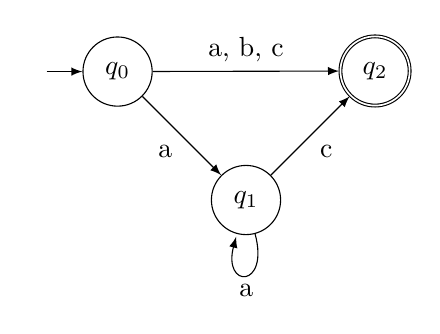
\begin{tikzpicture}[initial text={}, >={latex}]
    \node[state, initial]     (q_0)                         {$q_0$};
    \node[state]              (q_1)   [below right=of q_0]  {$q_1$};
    \node[state, accepting]   (q_2)   [above right=of q_1]  {$q_2$};
    \path[->] (q_0) edge              node [below left]   {a} (q_1)
              (q_1) edge [loop below] node [below]        {a} (q_1)
              (q_1) edge              node [below right]  {c} (q_2)
              (q_0) edge              node [above]  {a, b, c} (q_2);
  \end{tikzpicture}
  
  \caption{an NFA accepting the language $\{a, b, c\} \cup \{a\}\{a\}^*\{c\}$}
  \label{fig:nfa_a+b+a*c}
\end{figure}

Is the word $aaac$ accepted by this automaton?
\begin{align*}
  (\{q_0\}, aaac) & \vdash (\{q_1, q_2\}, aac) \\
  & \vdash (\{q_1\}, ac) \\
  & \vdash (\{q_1\}, c) \\
  & \vdash (\{q_2\}, \epsilon)
\end{align*}
Since the state $q_2$ is final, and the configuration ends with $\epsilon$, the word $aaac$ is accepted. It is important to note that there are infinitely many NFAs representing the same language. We will therefore focus our attention on efficient ways to construct NFAs that avoid needlessly large machines.

The definition of an NFA can be extended to allow empty transitions of the form $(p, \epsilon, q)$ for some states $p, q$. Allowing $\epsilon$-transitions simplifies some algorithms considered in this paper, but does not result in a more powerful language describing method. That is, NFAs without $\epsilon$-transitions (called \emph{$\epsilon$-free} or \emph{sequential}) can express exactly the same languages as NFAs with $\epsilon$-transitions. In Section \ref{sec:Empty Removal Construction} we define a construction that removes $\epsilon$-transitions from an NFA, and leaves a sequential NFA. Any NFA with an empty transition $(p, \epsilon, q)$ at state $p$ may move to state $q$ without consuming any symbols from the input word.

For any regular expression, we can construct an NFA using the structural induction method - also known as the Thompson construction. This construction is illustrated in Figure \ref{fig:thompson construction}. There is always one initial and one final state, and previous subtree computations are joined together using $\epsilon$-transitions going into the initial state(s), and out of final state(s). 

The rest of this paper will use a consistent notation when illustrating various NFA construction methods. New states will be left unnamed, previously computed subtree NFAs will be drawn in an appropriate box, and any modifications to previously computed NFAs will be in bold. We define the following meanings for the names of states for all constructions illustrated in this paper:
\begin{center}
  \begin{tabular}{r|l}
    State Name & Meaning \\
    \hline
    $i_\alpha$  & The initial state of NFA($\alpha$) \\
    $f_\alpha$  & The \emph{only} final state of NFA($\alpha$) \\
    $f^i_\alpha$ & The $i^{th}$ final state of NFA($\alpha$) \\
    $x, y$      & States $x$ and $y$ are merged
  \end{tabular}
\end{center}

\begin{figure}[H]
  \centering
  \begin{subfigure}[b]{0.4\linewidth}
    \centering
    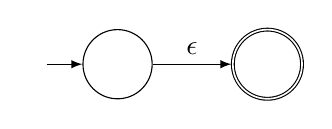
\begin{tikzpicture}[initial text={}, >={latex}]
      \node[state, initial]   (q_0)                {};
      \node[state, accepting] (q_1) [right=of q_0] {};
      \path[->] (q_0) edge node [above] {$\epsilon$} (q_1);
    \end{tikzpicture}
    \caption{Empty word}
  \end{subfigure}
  %
  \begin{subfigure}[b]{0.4\linewidth}
    \centering
    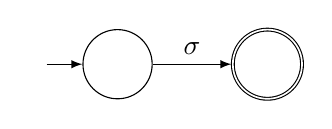
\begin{tikzpicture}[initial text={}, >={latex}]
      \node[state, initial]   (q_0)                {};
      \node[state, accepting] (q_1) [right=of q_0] {};
      \path[->] (q_0) edge node [above] {$\sigma$} (q_1);
    \end{tikzpicture}
    \caption{Atom $\sigma$}
  \end{subfigure}
  
  \vspace{1cm}
  
  \begin{subfigure}[b]{0.5\linewidth}
    \centering
    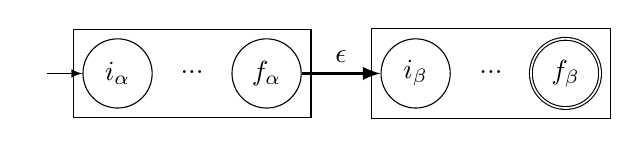
\begin{tikzpicture}[initial text={}, >={latex}]
      \node[state, initial]   (q_0)                 {$i_\alpha$};
      \node[state]            (q_1) [right=of q_0]  {$f_\alpha$};
      \node[state]            (q_2) [right=of q_1]  {$i_\beta$};
      \node[state, accepting] (q_3) [right=of q_2]  {$f_\beta$};
      \node[draw, fit={(q_0)(q_1)}]                 {...};
      \node[draw, fit={(q_2)(q_3)}]                 {...};
      \path[->] (q_1) edge [very thick] node [above] {$\epsilon$} (q_2);
    \end{tikzpicture}
    \caption{Concatenation $(\alpha \beta)$}
  \end{subfigure}
  
  \vspace{1cm}
  
  \begin{subfigure}[b]{0.4\linewidth}
    \centering
    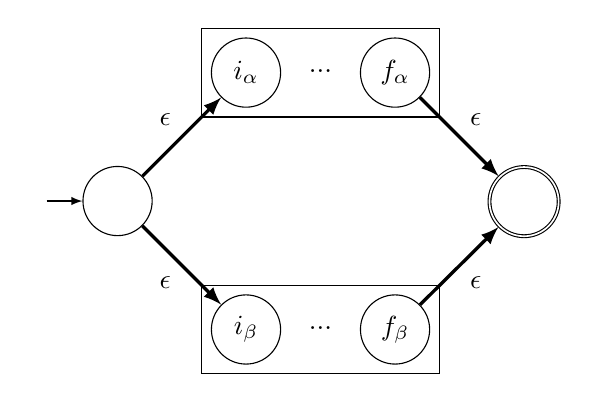
\begin{tikzpicture}[initial text={}, >={latex}]
      \node[state, initial]   (q_0)                       {};
      \node[state]            (q_1) [above right=of q_0]  {$i_\alpha$};
      \node[state]            (q_2) [right=of q_1]        {$f_\alpha$};
      \node[state]            (q_3) [below right=of q_0]  {$i_\beta$};
      \node[state]            (q_4) [right=of q_3]        {$f_\beta$};
      \node[state, accepting] (q_5) [below right=of q_2]  {};
      \node[draw, fit={(q_1)(q_2)}] {...};
      \node[draw, fit={(q_3)(q_4)}] {...};
      \path[->] (q_0) edge [very thick] node [above left]  {$\epsilon$}  (q_1)
                (q_0) edge [very thick] node [below left]  {$\epsilon$}  (q_3)
                (q_2) edge [very thick] node [above right] {$\epsilon$}  (q_5)
                (q_4) edge [very thick] node [below right] {$\epsilon$}  (q_5);
    \end{tikzpicture}
    \caption{Disjunction $(\alpha + \beta)$}
  \end{subfigure}
  %
  \begin{subfigure}[b]{0.5\linewidth}
    \centering
    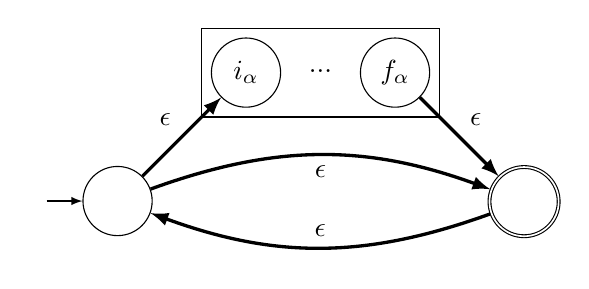
\begin{tikzpicture}[initial text={}, >={latex}]
      \node[state, initial]   (q_0)                       {};
      \node[state]            (q_1) [above right=of q_0]  {$i_\alpha$};
      \node[state]            (q_2) [right=of q_1]        {$f_\alpha$};
      \node[state, accepting] (q_3) [below right=of q_2]  {};
      \node[draw, fit={(q_1)(q_2)}] {...};
      \path[->] (q_0) edge [very thick] node [above left]            {$\epsilon$} (q_1)
                (q_2) edge [very thick] node [above right]           {$\epsilon$} (q_3)
                (q_0) [bend left=20, very thick] edge node [below]  {$\epsilon$} (q_3)
                (q_3) [bend left=20, very thick] edge node [above]  {$\epsilon$} (q_0);
    \end{tikzpicture}
    \caption{Star $\alpha^*$}
  \end{subfigure}
  \caption{Thompson construction}
  \label{fig:thompson construction}
\end{figure}
The optional operation case $\alpha?$ is omitted in this construction (and all others in this paper) because it is directly equivalent to $(\alpha + \epsilon)$ and can easily be handled as such. This construction shows that every mathematical regular expression can be converted into an NFA accepting the same language. The converse is also true using the state-removal construction, but the resulting regular expression is exponentially long, and the process is generally not useful in practice since developers typically write regular expressions and not NFAs.






\section{Empty Removal Construction}
\label{sec:Empty Removal Construction}
In general, NFAs are permitted to include $\epsilon$-transitions. But for some algorithms (see Section \ref{sec:Product Construction}) we require an NFA to have no $\epsilon$-transitions. Such an NFA is classified as \emph{sequential} or \emph{$\epsilon$-free}. Clearly, every sequential NFA is an NFA, but below we show an algorithm proving every NFA is also a sequential NFA.

To construct a sequential NFA $M'$ from NFA $M$, first copy all states and non-empty transitions. Define the function:
\begin{center}
  $E_M(q) = \{p : p \in Q, p \ne q$, and $p$ is reachable from $q$ using only $\epsilon$-transitions\}
\end{center}
Then for every state $q$ with outgoing transition $(q, a, p) \in \delta$, add transitions $\forall r \in E_M(p): (q, a, r)$ to $M'$. The initial state of $M'$ is the initial state of $M$, and the final states of $M'$ are $\forall f \in F: E_M(f)$.





\section{Product Construction}
\label{sec:Product Construction}
The algorithms available to NFAs are more well developed than algorithms for regular expressions. The product construction takes the intersection of two regular languages by taking sequential NFAs $A_1$ and $A_2$ and returning the NFA $M$ such that $L(M) = L(A_1) \cap L(A_2)$. The idea is to label each state in $M$ as a pair of states $(p, q)$ where $p \in A_1.Q$ and $q \in A_2.Q$. The initial state of $M$ is the pair of states where both elements are the initial state in their respective automaton - $(p_0, q_0)$. Any state in $M$ labelled $(p, q)$ is final if and only if $p \in A_1.F$ and $q \in A_2.F$.

Begin this algorithm by creating state in $M$ $(p_0, q_0)$ where $p_0$ is the initial state in $A_1$, and $q_0$ is the initial state in $A_2$. While there is some state not marked done $(p_i, q_n) \in M.Q$, take the intersection of every transition $(p_i, \alpha, p_j) \in A_1.\delta$ with every transition $(q_n, \beta, q_m) \in A_2.\delta$: if $\alpha = \beta$, add state $(p_j, q_m)$ to $M$ if it does not exist, and add transition $((p_i, q_n), \alpha, (p_j, q_m))$ to $M$. Once every outgoing transition pair from state $(p_i, q_n)$ is fully explored, mark the state as done. Finally, make each state $(p, q)$ final in $M$ if and only if both $p \in A_1.F$ and $q \in A_2.F$.

For example, suppose there were two NFAs $P$ and $Q$ from Figure \ref{fig:product construction example}. Using the product construction, a new NFA is created that accepts exactly the language $L(P) \cap L(Q)$.

\begin{figure}[H]
  \begin{subfigure}[b]{0.5\linewidth}
    \centering
    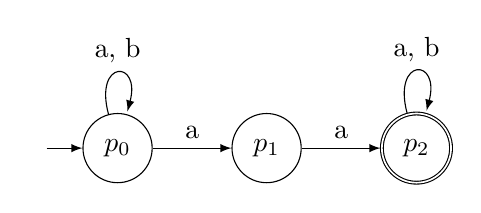
\begin{tikzpicture}[initial text={}, >={latex}]
      \node[state, initial]   (p0)               {$p_0$};
      \node[state]            (p1) [right=of p0] {$p_1$};
      \node[state, accepting] (p2) [right=of p1] {$p_2$};
      \path[->] (p0) edge [loop above] node [above] {a, b}  (p0)
                (p2) edge [loop above] node [above] {a, b}  (p2)
                (p0) edge              node [above] {a}     (p1)
                (p1) edge              node [above] {a}     (p2);
    \end{tikzpicture}
    \caption{NFA $P$ accepting all words with the substring $aa$}
  \end{subfigure}
  %
  \begin{subfigure}[b]{0.5\linewidth}
    \centering
    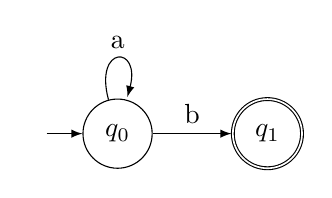
\begin{tikzpicture}[initial text={}, >={latex}]
      \node[state, initial]   (q0)               {$q_0$};
      \node[state, accepting] (q1) [right=of q0] {$q_1$};
      \path[->] (q0) edge [loop above] node [above] {a} (q0)
                (q0) edge              node [above] {b} (q1);
    \end{tikzpicture}
    \caption{NFA $Q$ accepting all words of the form $(a^*b)$}
  \end{subfigure}
  
  \vspace{1cm}
  
  \begin{subfigure}[b]{\linewidth}
    \centering
    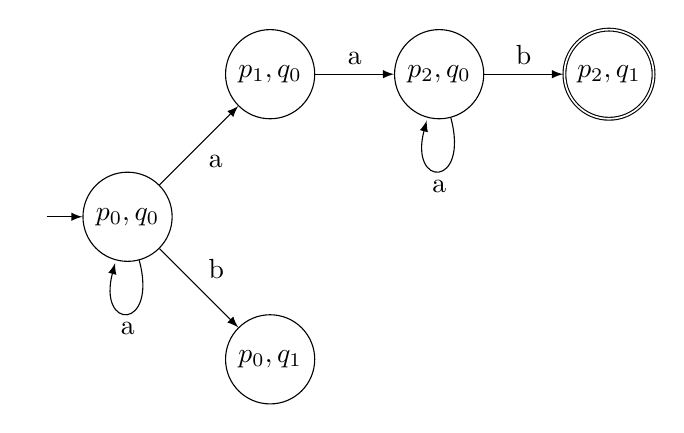
\begin{tikzpicture}[initial text={}, >={latex}]
      \node[state, initial]   (00)                      {$p_0,q_0$};
      \node[state]            (01) [below right=of 00]  {$p_0,q_1$};
      \node[state]            (10) [above right=of 00]  {$p_1,q_0$};
      \node[state]            (20) [right=of 10]        {$p_2,q_0$};
      \node[state, accepting] (21) [right=of 20]        {$p_2,q_1$};
      \path[->] (00) edge [loop below] node [below]       {a} (00)
                (00) edge              node [above right] {b} (01)
                (00) edge              node [below right] {a} (10)
                (10) edge              node [above]       {a} (20)
                (20) edge [loop below] node [below]       {a} (20)
                (20) edge              node [above]       {b} (21);
    \end{tikzpicture}
    \caption{Product-constructed NFA accepting exactly $L(P) \cap L(Q)$}
  \end{subfigure}

  \caption{Product construction example with $\Sigma = \{a, b\}$}
  \label{fig:product construction example}
\end{figure}

The product construction becomes extremely useful with respect to the language enumeration problem in Section \ref{sec:Regular Language Enumeration}.





\section{Context-Free Grammars}
\label{sec:Context-Free Grammars}
Context-free grammars (CFG) are a more powerful encoding of formal languages than mathematical regular expressions and finite automata. Formally, they are defined as a 4-tuple: ($\Gamma$, $\Sigma$, $R$, $S$) where $\Gamma$ is a set of non-terminal symbols, $\Sigma$ is the alphabet (set of terminal symbols), $R$ is a set of production rules of the form $\gamma \in \Gamma \rightarrow (\Gamma \cup \Sigma)^*$, and $S$ is the start symbol $\in \Gamma$. Note that $\Gamma$ and $\Sigma$ are disjoint sets. Any language described by a CFG is considered a \emph{context-free language}. 

Regular languages are a proper subset of context-free languages; any regular language represented by NFA $M$ can be expressed using a CFG $G$ with the following approach: 
\begin{enumerate}
  \item The non-terminals of $G$ are the state names of $M$.
  \item The start symbol of $G$ is the initial state of $M$.
  \item For every transition $(P, \sigma, Q) \in M.\delta$, add to $G$ the rule $P \rightarrow \sigma Q$.
  \item For every final state $F \in M.F$, add to $G$ the rule $F \rightarrow \epsilon$.
\end{enumerate} 
Using the pumping lemma, we can prove certain languages are context-free but not regular. Take for example the language of balanced parentheses defined by the context-free grammar:
\begin{center}
  $(\{S\}, \{(, )\}, \{S \rightarrow SS, S \rightarrow (S), S \rightarrow \epsilon\}, S)$  
\end{center}
There is no such representation using mathematical regular expressions or NFAs. Many important languages are also context-free but not regular, such as most source code, regular expression strings, arithmetic expressions, and binary trees. Context-free languages can recurse into themselves; this is a useful property missing from regular languages.

A \emph{derivation} is a sequence of production rule applications yielding a word. Any derivable word is accepted/generated by the CFG. Using the balanced parentheses language defined above, the word ()(()) is shown to be a member of this language through the derivation: 
\begin{center}
  $S \Rightarrow SS \Rightarrow (S)S \Rightarrow ()S \Rightarrow ()(S) \Rightarrow ()((S)) \Rightarrow ()(())$  
\end{center}
Equivalently, this derivation generates the parse tree shown in Figure \ref{fig:bp_tree}. The \emph{yield} is the concatenation of the leaves from left to right.

\begin{figure}[H]
  \centering
  \Tree 
  [
    .S
    [
      .S 
      [
        ( 
        [
          .S 
          $\epsilon$ 
        ] 
        ) 
      ]
    ]
    [
      .S 
      [
        ( 
        [
          .S 
          [
            ( 
            [
              .S 
              $\epsilon$ 
            ] 
            ) 
          ]
        ] 
        ) 
      ]
    ]
  ]
  \caption{Parse tree of ``()(())'' using the balanced parentheses grammar.}
  \label{fig:bp_tree}
\end{figure}




















  \chapter{Literature Review}
  \label{ch:Literature Review}
  This section aims to explore concepts that are less widely known among researchers outside the area of regular languages. Along with summarizing the important task of language enumeration algorithms, this section also outlines the backtracking membership algorithm, as well as Glushkov, position, partial derivative, and follow constructions for converting a regular expression into an NFA.


\section{Regular Language Enumeration}
\label{sec:Regular Language Enumeration}
In order to test the efficiency of regular expression membership algorithms, we need to generate words accepted by the regular expression. This is the language enumeration problem, and it can be approached with respect to the regular expression tree as well as an equivalent NFA.

\subsection{Pairwise Word Generation}
\label{subsec:Pairwise Word Generation}
Word generation applied directly onto a regular expression tree is approached as a finite set construction by Zheng et al \cite{pairgen}. One of the main advantages of regular expressions allows the representation of infinite languages using the star operator, so to generate a finite set of words we must limit the number of repetitions allowed of each star. That is, each $(r^*)$ becomes $(r^0 + r^1 + ... + r^k)$ for some integer $1 < k < \infty$. \emph{Combination coverage} is the simplest way to generate words, since we rely on enumerating every word in the language. Its implementation is simple, depending on the structure of each node on the tree. For a regular expression $r$, generate the combination coverage set by calling $C(r)$.

\begin{enumerate}
  \item $C(\alpha \beta) = C(\alpha) C(\beta)$
  \item $C(\alpha + \beta) = C(\alpha) \cup C(\beta)$
  \item $C(\alpha^*) = C(\alpha)^0 \cup C(\alpha)^1 \cup ... \cup C(\alpha)^k$
  \item $C(\alpha?) = \{\epsilon\} \cup C(\alpha)$
  \item $C(\epsilon) = \{\epsilon\}$
  \item $C(\sigma\in\Sigma) = \{\sigma\}$ 
  \item $C( [...\sigma_0-\sigma_1...\sigma_2...]) = ... \cup \{\sigma : \sigma_0 \leq \sigma \leq \sigma_1\} \cup ... \cup \{\sigma_2\} \cup ...$ \\
      (Every symbol accepted by the character class)
\end{enumerate}

However, combination coverage returns an excessive number of words. Not only is this computationally expensive to create (both in time and memory), but a complete set of words is too large when testing an arbitrary regular expression \cite{pairgen}. To limit the number of words, \emph{pairwise} word generation is employed. Pairwise testing applies generally to software where there is a set of variables, each with a finite number of assignments. With combination testing, we test every possible combination of variable assignment. Whereas with pairwise testing we are only concerned with testing pairs of variable assignments \cite{pairwise}. The key idea is to test multiple paired assignments simultaneously.

For the regular expression $r = (a+b)(c+d)(e+f)$, combination coverage enumerates the entire language $|L(r)|=8$. But pairwise coverage is achieved with the set $\{ace, ade, adf, bcf, bde\} \subset L(r)$. This means that every paired combination of assignments is seen in this subset (i.e., $a$ is paired with all $c, d, e, f$; $c$ is paired with all $a,b,e,f$; etc.). Pairwise coverage requires five words, whereas combination coverage requires eight. These savings grow as the regular expression gains complexity.

FAdo implements binary concatenations. This improves simplicity across many algorithms, but totally destroys any savings seen through pairwise concatenation since binary concatenation is pairwise by definition. Instead, we use combination coverage and attempt to limit the number of test cases through problem-specific assumptions:

\begin{enumerate}
  \item $C(.) =$ 16 arbitrarily chosen ASCII symbols
  \item $C([...a-b...c...]) = \{a, b, \sigma, c, ...\}$ for some $\sigma$ between $a,b$
  \item $C(\alpha\beta) =$ no more than 10,000 words sampled randomly (with constant seed) from all possibilities
  \item $C(\alpha^*) = \{\epsilon\} \cup C(\alpha) \cup G$ where $G$ is generated by identifying every pair that needs to be covered, and greedily concatenating them together. We also implemented a hard-limit that helps mitigate against $G$ from containing extremely long words.
    \begin{enumerate}
      \item If $\alpha = (a+b+c)$, which accepts $\{a, b, c\}$, then all \\
          $\{(a,a), (a,b), (a,c), (b,a), (b,b), (b,c), (c,a), (c,b), (c,c)\}$ pairs need to be covered.
      \item Begin arbitrarily with $aa$, then find any pair not yet covered that starts with an $a$. Say, $(a,b)$. The current word being built is now $aab$.
      \item Repeat, but looking for a pair starting with $b$: $(b, a)$. Now the word is $aaba$.
      \item Repeat, but looking for a pair starting with $a$: $(a, c)$. Now the word is $aabac$. \\
            Only the following pairs remain: $\{(b,b), (b,c), (c,a), (c,b), (c,c)\}$.
      \item Continue building the current word until a certain maximum number of repetitions is taken, no more pairs start with the desired letter, or all pairs are used.
      \item Note that in general, letters $a, b, c$ are words of any length.
    \end{enumerate}
\end{enumerate}

\subsection{NFA Language Enumeration}
\label{NFA Language Enumeration}
The other way to enumerate a regular expression $r$ and generate the language $L(r)$ is to construct a sequential NFA $M$ such that $L(M) = L(r)$, and use the  membership algorithm to generate words in lexicographic order. This approach allows a star operation to be maintained as a star operation, instead of having to limit its repetition. 

Consider any sequential NFA construction as the function $A(r)$ (e.g., the Thompson construction with empty-removal construction applied immediately after). The NFA enumeration algorithm describes how to enumerate cross-sections of a given NFA, where the $n^{th}$ cross-section of an NFA is the set of words of length $n$ accepted by the NFA. We use the product construction to construct the acyclic NFA $M_n = A(r) \cap A(.^n)$ where every path from the initial state is of length $n$. First, find the minimal word of $M_n$ by starting at the initial state and greedily taking minimum transitions; concatenate the minimum transition labels, and consider all concatenated words that end in a final state. Given a minimum word $w$, find the next word by running $w$ through the membership algorithm, then backtracking through previous state configurations until the next minimum transition can be taken, then find the minimal word in $M_n$ starting at each potential backtracked state. The entire cross-section has been enumerated when the algorithm backtracks to the initial state from its maximal outgoing transition \cite{nfa-enum}. This process can be repeated for any desired cross-section $n$.





\section{Backtracking Membership Algorithm}
\label{sec:Backtracking Membership Algorithm}
In order for a regular expression implementation to support non-regular operations such as backreferences (as used in some programmer's regular expressions), they must forego typical membership algorithms. Regular languages can decide membership in polynomial time (both using partial derivatives and NFA matching). But after adding non-regular operations such as backreferences, only exponentially bound backtracking algorithms are known. Even using the backtracking algorithm on a mathematical regular expression (i.e., without backreferences) involves an exponential worst-case time complexity. Adding backreferences makes deciding the membership problem NP-complete, since word membership could be solved in (linear) polynomial time to the input word's length if a perfect guessing function was known. Backtracking algorithms consider one state at a time and allow saving additional information like matched groups, whereas regular algorithms consider all possible states at once and rely on collision of these states.

The backtracking membership algorithm can be viewed with respect to a regular expression tree, as well as an NFA \cite{cata-backtrack}. This thesis tests backtracking membership directly using regular expression trees, which avoids the polynomial NFA construction cost. Using generating functions, we are able to write a recursive backtracking algorithm for each type of regular expression node on the regular expression tree. This algorithm tracks the remaining suffix left to match. The $Match$ function returns an iterator of suffixes of the input word. If any substring from the $Match(r, w)$ iterator is empty (i.e., all of $w$ has been matched by $r$), then $r$ accepts $w$. To fit within the scope of the rest of this paper, our implementation of the backtracking algorithm  only supports structures defined in mathematical regular expressions.

\begin{lstlisting}[label={alg:backtracking}, caption={Deciding membership using backtracking}]
Algorithm Backtrack Match($r$, $w$):
    if $r = \alpha\beta$:
        for $s$ in Match($\alpha$, $w$):
            for $s'$ in Match($\beta$, $s$):
                yield $s'$
    else if $r = \alpha|\beta$:
        for $s$ in Match($\alpha$, $w$):
            yield $s$
        for $s$ in Match($\beta$, $w$):
            yield $s$
    else if $r = \alpha^*$:
        for $s$ in Match($\alpha$, $w$):
            for $s'$ in Match($r$, $s$):
                yield $s'$
        yield $w$
    else if $r = \alpha?$:
        for $s$ in Match($\alpha$, $w$):
            yield $s$
        yield $w$
    else if $r = \epsilon$:
        yield $w$
    else if $r = \sigma$ or $r = [...\sigma...]$ or $r = .$:
        yield $\epsilon$
\end{lstlisting}

Algorithm \ref{alg:backtracking} is a modification of Algorithm 1 from \cite{cata-backtrack}, and has been adapted to fit within our mathematical regular expression specification implemented in FAdo. Figure \ref{fig:backtrack_demo}(a) shows the main pitfall of this simple membership algorithm: some words tested on vulnerable regular expressions will experience exponential membership time. In practice, regular expression libraries include many complicated optimizations to limit this exponential cost. Some mitigation strategies include optimizing the regular expression tree to avoid duplicate match options, or using memoization during word evaluation \cite{cata-backtrack, cox}.

\begin{figure}[H]
  \centering
  \begin{subfigure}[b]{0.45\linewidth}
    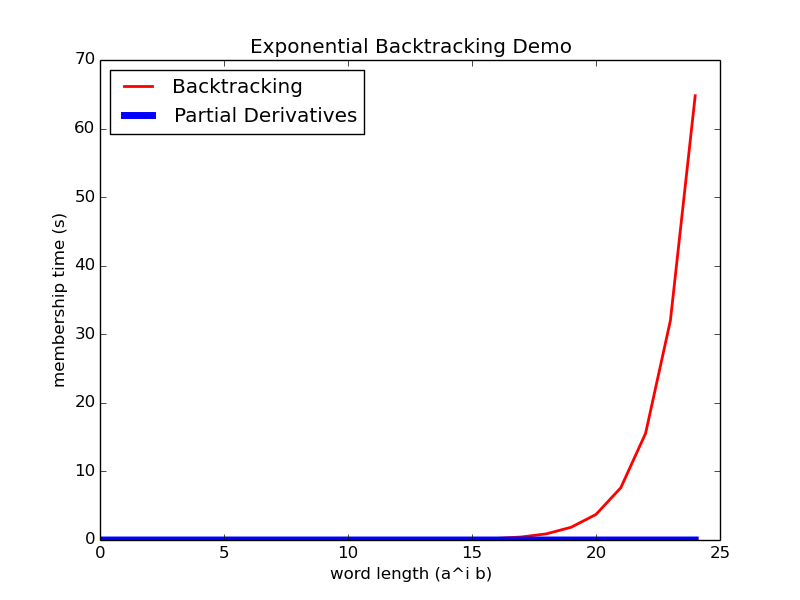
\includegraphics[width=\linewidth]{fig/backtrack_fado}
    \caption{Time to reject words $a^ib$, for $i\in\mathbb{N}$ in $(a+a)^*$ using backtracking vs. partial derivatives.}
  \end{subfigure}
  \hspace{1cm}
  \begin{subfigure}[b]{0.45\linewidth}
    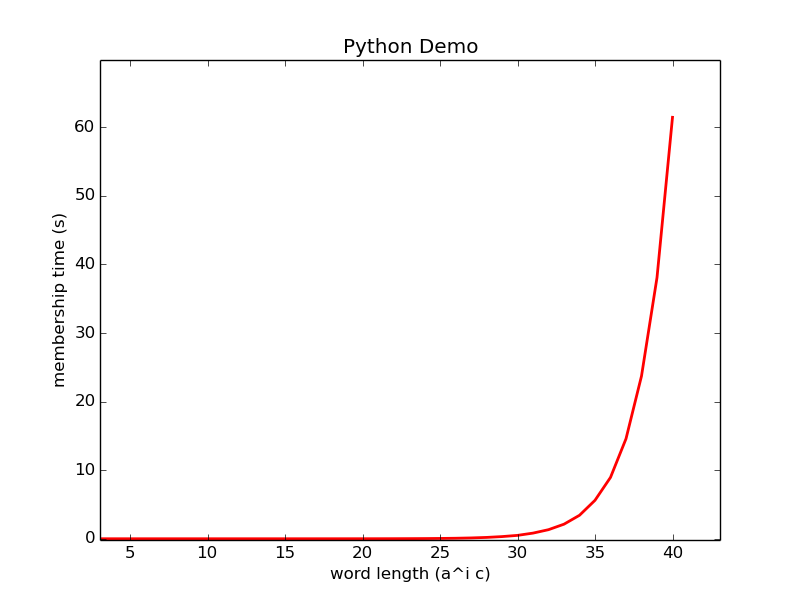
\includegraphics[width=\linewidth]{fig/backtrack_python}
    \caption{Time to reject words $a^ic$, for $i\in\mathbb{N}$ in $(a|aa)^*b$ using Python's built-in re module.}
  \end{subfigure}
  
  \caption{Backtracking suffers from exponential membership time}
  \label{fig:backtrack_demo}
\end{figure}

However, when using a carefully chosen regular expression that avoids structural optimizations, we are able to see exponential growth despite any internal memoization. Figure \ref{fig:backtrack_demo}(b) shows how Python's built-in re module is vulnerable to exponential membership time. This can lead to security vulnerabilities in any application that generates regular expressions based on user input, or uses regular expressions susceptible to a large amount of backtracking (like in Figure \ref{fig:backtrack_demo}). Theoretically, an attacker could launch a backtracking search capable of denying service to other users for hours \cite{cata-backtrack}. Such an attack is referred to as ReDoS (regular expression denial of service).






\section{Glushkov/Position NFA}
\label{sec:Glushkov/Position NFA}
The Glushkov and position constructions are two distinct approaches that build the same NFA. Some authors refer to this NFA as the Glushkov NFA while others call it the position NFA. The Glushkov construction \cite{glushkov-yu} algorithm can be thought of as the Thompson construction without the empty transitions, and potentially with multiple final states. Let states named $p_\alpha$ and $q_\alpha$ be successors of the initial state $i_\alpha$ of a given NFA $\alpha$. For concatenation, each state $f^i_\alpha$ is final if and only if $i_\beta$ is final, then for every transition $(i_\beta, \sigma, p_\beta)$, add transitions $(f^i_\alpha, \sigma, p_\beta)$. Disjunction simply merges the initial states. And star takes a similar approach to concatenation, but without creating any new states and making $i_\alpha$ final. Through every operation, the initial state only has outgoing transitions.

\begin{figure}[H]
  \centering
  \begin{subfigure}[b]{0.22\linewidth}
    \centering
    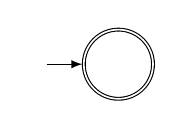
\begin{tikzpicture}[initial text={}, >={latex}]
      \node[state, initial, accepting] (0) {};
    \end{tikzpicture}
    \caption{Empty word}
  \end{subfigure}
  %
  \begin{subfigure}[b]{0.22\linewidth}
    \centering
    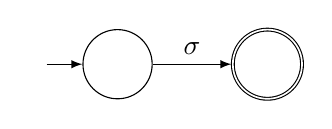
\begin{tikzpicture}[initial text={}, >={latex}]
      \node[state, initial]   (0)                {};
      \node[state, accepting] (1) [right=of 0] {};
      \path[->] (0) edge node [above] {$\sigma$} (1);
    \end{tikzpicture}
    \caption{Atom $\sigma$}
  \end{subfigure}
  %
  \begin{subfigure}[b]{0.45\linewidth}
    \centering
    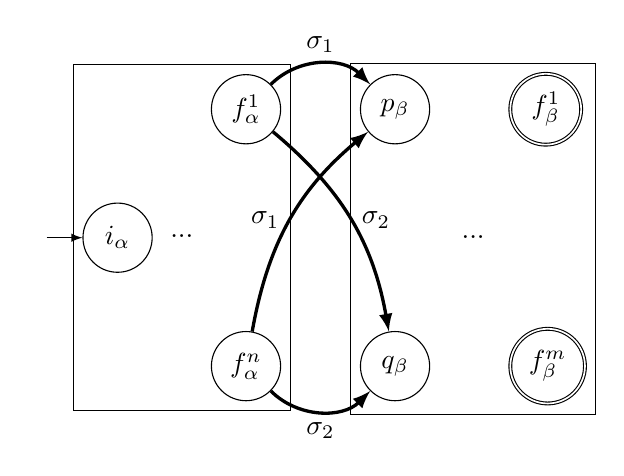
\begin{tikzpicture}[initial text={}, >={latex}]
      \node[state, initial]   (a0)                      {$i_\alpha$};
      \node[state]            (a1)  [above right=of a0] {$f^1_\alpha$};
      \node[state]            (an)  [below right=of a0] {$f^n_\alpha$};
      \node[draw, fit={(a0)(a1)(an)}]                   {...};      
      \node[state]            (p)   [right=of a1]       {$p_\beta$};
      \node[state]            (q)   [right=of an]       {$q_\beta$};
      \node[state, accepting] (b1)  [right=of p]        {$f^1_\beta$};
      \node[state, accepting] (bn)  [right=of q]        {$f^m_\beta$};
      \node[draw, fit={(p)(q)(b1)(bn)}]                 {...};
      \path[->] (a1) edge [bend left=45, very thick] node [above] {$\sigma_1$} (p)
                (a1) edge [bend left=20, very thick] node [right] {$\sigma_2$} (q)
                (an) edge [bend left=20, very thick] node [left]  {$\sigma_1$} (p)
                (an) edge [bend right=45, very thick] node [below]{$\sigma_2$} (q);
    \end{tikzpicture}
    \caption{Concatenation $(\alpha \beta)$}
  \end{subfigure}
  
  \vspace{1cm}
  
  \begin{subfigure}[b]{0.45\linewidth}
    \centering
    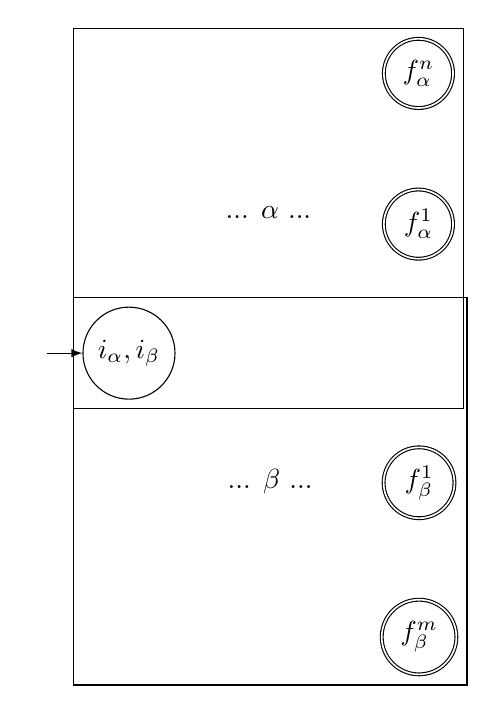
\begin{tikzpicture}[initial text={}, >={latex}]
      \node[state, initial]   (0)                     {$i_\alpha, i_\beta$};
      \node[state, draw=none] (n) [right=of 0]        {};
      \node[state, accepting] (f1) [above right=of n] {$f^1_\alpha$};
      \node[state, accepting] (f2) [above=of f1]      {$f^n_\alpha$};
      \node[state, accepting] (f3) [below right=of n] {$f^1_\beta$};
      \node[state, accepting] (f4) [below=of f3]      {$f^m_\beta$};
      \node[draw, fit={(0)(f1)(f2)}] {... $\alpha$ ...};
      \node[draw, fit={(0)(f3)(f4)}] {... $\beta$ ...};
    \end{tikzpicture}
    \caption{Disjunction $(\alpha + \beta)$}
  \end{subfigure}
  %
  \begin{subfigure}[b]{0.45\linewidth}
    \centering
    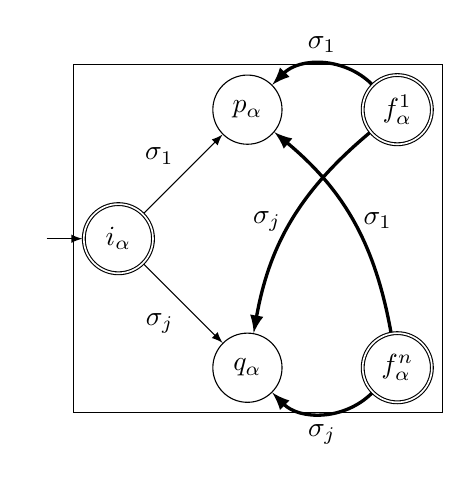
\begin{tikzpicture}[initial text={}, >={latex}]
      \node[state, initial, accepting] (0)                     {$i_\alpha$};
      \node[state]            (1) [above right=of 0]  {$p_\alpha$};
      \node[state]            (2) [below right=of 0]  {$q_\alpha$};
      \node[state, accepting] (3) [right=of 1]        {$f^1_\alpha$};
      \node[state, accepting] (4) [right=of 2]        {$f^n_\alpha$};
      \node[draw, fit={(0)(1)(2)(3)(4)}]              {};
      \path[->] (0) edge node [above left] {$\sigma_1$} (1)
                (0) edge node [below left] {$\sigma_j$} (2)
                (3) edge [very thick, bend right=45] node [above] {$\sigma_1$} (1)
                (3) edge [very thick, bend right=20] node [left]  {$\sigma_j$} (2)
                (4) edge [very thick, bend right=20] node [right] {$\sigma_1$} (1)
                (4) edge [very thick, bend left=45]  node [below] {$\sigma_j$} (2);
    \end{tikzpicture}
    \caption{Star $\alpha^*$}
  \end{subfigure}
  \caption{Glushkov construction}
  \label{fig:glushkov construction}
\end{figure}

Although the position automaton \cite{position} is identical to the Glushkov automaton, its construction is significantly different. To convert regular expression $r$ into an NFA using the position construction, we begin by uniquely \emph{marking} each atom in $r$ according to its left-to-right position. For example, the marked version of $a(b+a)b^*$ is $a_1(b_2+a_3)b_4^*$. Then informally define the following functions:

$first(r)$ is the set of marked atoms that could represent the first symbol in a matched word (e.g., $first(a_1(b_2+a_3)b_4^*) = \{a_1\}$). Similarly, $last(r)$ is the set of marked atoms that could represent the last symbol in a matched word (e.g., $last(a_1(b_2+a_3)b_4^*) = \{b_2, a_3, b_4\}$). Finally, $follow(r, \sigma_i)$ is the set of atoms directly reachable in $r$ from the atom $\sigma_i$ (e.g., $follow(a_1(b_2+a_3)b_4^*, b_2) = \{b_4\}$). Because the informal definition is so intuitive, the rigorous approach is not included as it only overcomplicates matters. Curious readers can refer to \cite{follow} for their inductive definitions.

These functions are used in three distinct phases of the position construction. 
First, create an initial state $i$, and for each element $\sigma_i$ in $first(r)$ create the state named $\sigma_i$ if it does not exist, and add transition $(i, \sigma, \sigma_i)$. Mark state $i$ as done.
Then, while there is some state $q_j$ in the NFA not marked as done: iterate through each $\sigma_i \in follow(r, q_j)$. Create the state $\sigma_i$ if it does not exist, and add a transition $(q_j, \sigma, \sigma_i)$ to the NFA, and mark state $\sigma_i$ as done.
Finally, make each state $\sigma_i \in last(r)$ final.





\section{Partial Derivative NFA}
\label{sec:Partial Derivative NFA}
At a high-level, the partial derivative automaton represents all partial derivative possibilities of a regular expression for every alphabet symbol. Each state is named by a regular expression, so the initial state is the original regular expression being encoded, and the final states are any state named $r$ where $\epsilon \in L(r)$. The transition $(p, \sigma, q)$ exists if and only if the set of partial derivatives of $p$ with respect to $\sigma$ includes $q$. That is, $q \in \delta_\sigma(p)$ as defined in Section \ref{sec:Derivatives}.

The approach from Antimirov \cite{Antimirov} defines the \emph{linear form} of a regular expression $p$ as the set of 2-tuples $\{(\sigma, q) : \sigma\in\Sigma, q\in\delta_\sigma(p)\}$. To convert regular expression $r$ into the partial derivative NFA: create a set of newly created states $N$ initialized to $\{r\}$. While there is some newly created state $p$ (representing a regular expression), compute the linear form and iterate through each $(\sigma, q)$ pair. If $q$ has not yet been created, add it to $N$ and create the state. Then for each pair, create the transition $(p, \sigma, q)$.

Because each state of the partial derivative NFA represents a partial derivative derivable from the root $r$ of the regular expression tree, and $pd(r) \leq |r|_\Sigma$, the partial derivative NFA can have no more than $|r|_\Sigma$ states \cite{Antimirov}. This leads to the partial derivative NFA generally having fewer states than other constructions. Additionally, the partial derivative automaton is a quotient of the position automaton; meaning the position automaton can be converted into the partial derivative automaton by merging some states. Figure \ref{fig:nfaPD p tag} illustrates this point with an example using the regular expression accepting HTML paragraph tags. While the partial derivative NFA for this regular expression is of size 13, the Thompson construction creates an NFA of size 50 (omitted due to its large size).

\begin{figure}[H]
  \centering
  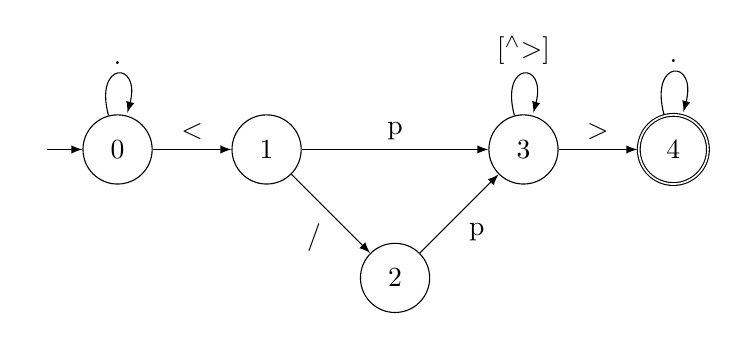
\begin{tikzpicture}[initial text={}, >={latex}]
    \node[state, initial]   (0)                     {0};
    \node[state]            (1) [right=of 0]        {1};
    \node[state]            (2) [below right=of 1]  {2};
    \node[state]            (3) [above right=of 2]  {3};
    \node[state, accepting] (4) [right=of 3]        {4};
    \path[->] (0) edge [loop above] node [above]        {$.$}           (0)
              (0) edge              node [above]        {$<$}           (1)
              (1) edge              node [below left]   {/}             (2)
              (1) edge              node [above]        {p}             (3)
              (2) edge              node [below right]  {p}             (3)
              (3) edge [loop above] node [above]        {$[^\wedge >]$} (3)
              (3) edge              node [above]        {$>$}           (4)
              (4) edge [loop above] node [above]        {$.$}           (4);
  \end{tikzpicture}
  \caption{Partial derivative NFA of the expression $.^*(</?p[^\wedge >]>).^*$}
  \label{fig:nfaPD p tag}
\end{figure}

Finding the linear form of a regular expression is costly, especially for large trees. A simple memoization approach lessens the amount of work needed by only computing the linear form for each recursively defined regular expression once, and saving it for future use. This optimized approach is implemented as the ``nfaPDO'' algorithm within FAdo, while the repetitive version is simply ``nfaPD''.

Even when using the optimized construction, the partial derivative automaton was very slow to construct for longer regular expressions until the nfaPDDAG (partial derivative directed acyclic graph) algorithm was published \cite{pddag}. The nfaPDDAG algorithm works by transforming the regular expression tree into a compressed regular expression directed acyclic graph (DAG) without duplicate subtrees; where each node of the compressed regular expression tree is created in the DAG and is uniquely assigned with an increasing index. Each node has no knowledge of the exact regular expression it represents, and instead stores information if the regular expression would have accepted the empty word, and outgoing labelled transitions and their node indices. Once the DAG is constructed, it can be easily converted into an NFA by starting with the root node/index and propagating according to the outgoing labelled transitions.

This algorithm is very fast because it compresses the regular expression (no longer re-computing multiple times for the same subtree in different locations), and uses integer hashing instead of tree hashing. As implemented in FAdo, regular expression tree hashing first converts the tree into a string, then hashes the string using Python's built-in hash function. Tree hashing has a linear cost with the size of the tree, while integer hashing can be done in constant time.





\section{Follow NFA}
\label{sec:Follow NFA}
The follow automaton was first presented by Lucian Ilie and Sheng Yu in 2003 \cite{follow}. In their paper they presented two new automata constructions for regular expression $\alpha$: $A_{follow}^\epsilon(\alpha)$ that constructs an NFA with empty transitions, and $A_{follow}(\alpha)$ that efficiently removes empty transitions from $A_{follow}^\epsilon(\alpha)$. Building $A_{follow}^\epsilon(\alpha)$ for regular expression $\alpha$ is defined inductively, similar to the Thompson construction from Section \ref{sec:Finite Automata}, and is also implemented within FAdo as ``nfaFollowEpsilon'' \cite{fado}.

\begin{figure}[H]
  \centering
  \begin{subfigure}[b]{0.22\linewidth}
    \centering
    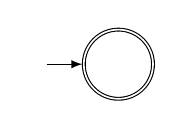
\begin{tikzpicture}[initial text={}, >={latex}]
      \node[state, initial, accepting]   (q_0) {};
    \end{tikzpicture}
    \caption{Empty word}
  \end{subfigure}
  %
  \begin{subfigure}[b]{0.22\linewidth}
    \centering
    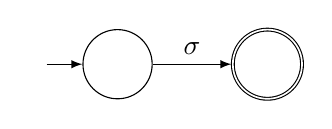
\begin{tikzpicture}[initial text={}, >={latex}]
      \node[state, initial]   (q_0)                {};
      \node[state, accepting] (q_1) [right=of q_0] {};
      \path[->] (q_0) edge node [above] {$\sigma$} (q_1);
    \end{tikzpicture}
    \caption{Atom $\sigma$}
  \end{subfigure}
  %
  \begin{subfigure}[b]{0.45\linewidth}
    \centering
    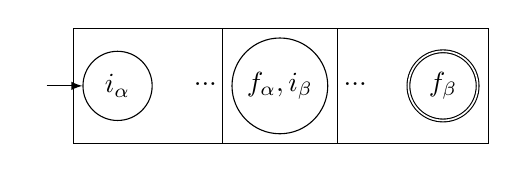
\begin{tikzpicture}[initial text={}, >={latex}]
      \node[state, initial]   (q_0)                 {$i_\alpha$};
      \node[state]            (q_1) [right=of q_0]  {$f_\alpha, i_\beta$};
      \node[state, accepting] (q_2) [right=of q_1]  {$f_\beta$};
      \node[draw, fit={(q_0)(q_1)}]                 {...};
      \node[draw, fit={(q_1)(q_2)}]                 {...};
    \end{tikzpicture}
    \caption{Concatenation $(\alpha \beta)$}
  \end{subfigure}
  
  \vspace{1cm}
  
  \begin{subfigure}[b]{0.45\linewidth}
    \centering
    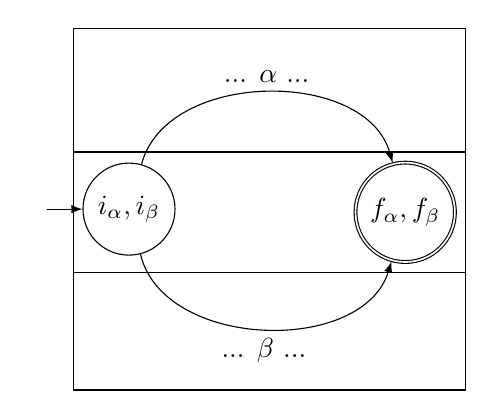
\begin{tikzpicture}[initial text={}, >={latex}]
      \node[state, initial]   (q_0)                      {$i_\alpha, i_\beta$};
      \node[state, draw=none] (qa)  [above right=of q_0] {};
      \node[state, accepting] (q_1) [below right=of qa]  {$f_\alpha, f_\beta$};
      \node[state, draw=none] (qb)  [below right=of q_0] {};
      \node[draw, fit={(q_0)(q_1)(qa)}]                  {};
      \node[draw, fit={(q_0)(q_1)(qb)}]                  {};
      \path[->] (q_0) edge [bend left=75]   node [above] {... $\alpha$ ...} (q_1)
                (q_0) edge [bend right=75]  node [below] {... $\beta$ ...}  (q_1);
    \end{tikzpicture}
    \caption{Disjunction $(\alpha + \beta)$}
  \end{subfigure}
  %
  \begin{subfigure}[b]{0.45\linewidth}
    \centering
    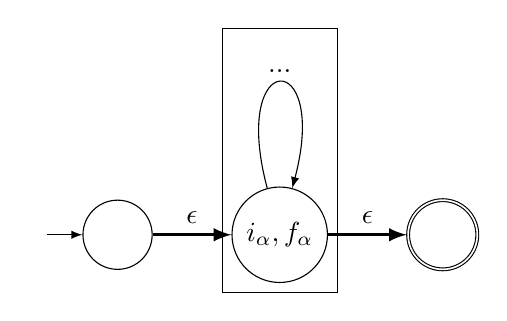
\begin{tikzpicture}[initial text={}, >={latex}]
      \node[state, initial]   (q_0)                 {};
      \node[state]            (q_1) [right=of q_0]  {$i_\alpha, f_\alpha$};
      \node[state, accepting] (q_2) [right=of q_1]  {};
      \node[state, draw=none] (qa)  [above=of q_1]  {};
      \node[draw, fit={(q_1)(qa)}]                  {};
      \path[->] (q_0) edge [very thick] node [above] {$\epsilon$} (q_1)
                (q_1) edge [very thick] node [above] {$\epsilon$} (q_2)
                (q_1) edge [loop above, looseness=15] node [above] {...} (q_1);
    \end{tikzpicture}
    \caption{Star $\alpha^*$}
  \end{subfigure}
  \caption{Follow construction (see below for additional instructions after each step)}
  \label{fig:follow construction}
\end{figure}

For each presented case, a post-processing step is completed to remove unnecessary empty transitions as they are created. 
\begin{itemize}
  \item Concatenation: merge state $f_\alpha, i_\beta$ with any state reachable through one or more \emph{undirected} empty transitions. That is, interpret every $\epsilon$-transition as going both ways.
  \item Star: if $i_\alpha, f_\alpha$ is involved in any cycle with only empty transitions, then all involved states are merged into $i_\alpha, f_\alpha$.
  \item Any case: if the initial state $i$ only has one outgoing transition of the form $(i, \epsilon, i')$, then $i$ is removed and $i'$ becomes the new initial state.
\end{itemize}

This construction is comparable to the Thompson NFA which also uses empty transitions; but the Thompson NFA is always larger. The true follow automaton uses a specialized empty removal construction to return a sequential NFA. The follow NFA is found to be a quotient of the position NFA \cite{follow}.

Although a general case of the empty removal construction is presented in Section \ref{sec:Empty Removal Construction}, the conversion from $A_{follow}^\epsilon(\alpha)$ to the sequential follow NFA $A_{follow}(\alpha)$ is performed in a specific order that improves efficiency. The states $Q$ of $A_{follow}^\epsilon(\alpha)$ are sorted in topological order $Q'$ according to the heuristic:
\begin{center}
  $p, q \in Q: p \leq q \texttt{ iff } (p, \epsilon, q) \in A_{follow}^\epsilon(\alpha).\delta$  
\end{center}
Then, the sorted set of states $Q'$ is considered in reverse order: for each transition $(q \in Q', \epsilon, p)$, find all transitions $(p, \sigma, r)$. Add the transition $(q, \sigma, r)$, remove the transition $(p, \sigma, r)$, and if state $p$ is final, then make $r$ final.

So far, the follow automaton may include disconnected, unreachable, or useless states from the initial state. To \emph{trim} these states, explore through the NFA starting at the initial state and mark any state as useful or not. A state is marked useful if it can be involved in a path from the initial state to any final state. Any unmarked or not useful state is removed along with any of its associated incoming/outgoing transitions. 

\begin{figure}[H]
  \centering
  \begin{subfigure}[b]{0.4\linewidth}
    \centering
    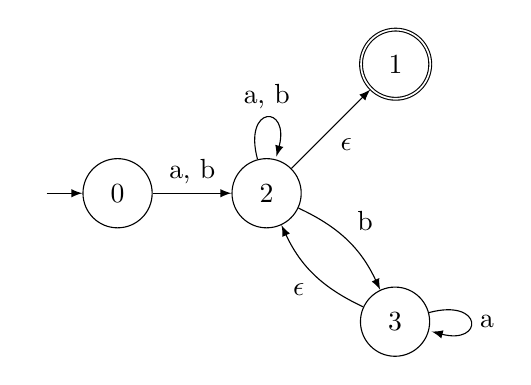
\begin{tikzpicture}[initial text={}, >={latex}]
      \node[state, initial]   (0)                     {0};
      \node[state]            (2) [right=of 0]        {2};
      \node[state]            (3) [below right=of 2]  {3};
      \node[state, accepting] (1) [above right=of 2]  {1};
      \path[->] (0) edge                node [above]      {a, b}       (2)
                (2) edge [loop above]   node [above]      {a, b}       (2)
                (2) edge                node [below right] {$\epsilon$} (1)
                (2) edge [bend left=20] node [above right] {b}         (3)
                (3) edge [loop right]   node [right]       {a}         (3)
                (3) edge [bend left=20] node [below left] {$\epsilon$} (2);
    \end{tikzpicture}
    \caption{$A_{follow}^\epsilon(\alpha)$}
  \end{subfigure}
  %
  \begin{subfigure}[b]{0.4\linewidth}
    \centering
    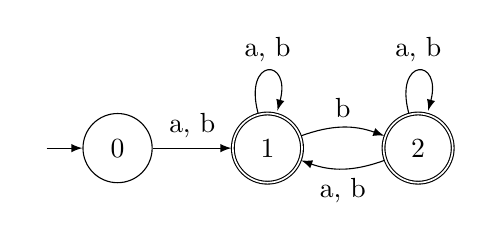
\begin{tikzpicture}[initial text={}, >={latex}]
      \node[state, initial]   (0)              {0};
      \node[state, accepting] (1) [right=of 0] {1};
      \node[state, accepting] (2) [right=of 1] {2};
      \path[->] (0) edge                node [above]      {a, b}    (1)
                (1) edge [loop above]   node [above]      {a, b}    (1)
                (1) edge [bend left=20] node [above]      {b}       (2)
                (2) edge [bend left=20] node [below]      {a, b}    (1)
                (2) edge [loop above]   node [above]      {a, b}    (2);
    \end{tikzpicture}
    \caption{$A_{follow}(\alpha)$}
  \end{subfigure}
  \caption{Follow construction example \cite{follow}}
  \label{fig:follow construction example}
\end{figure}

Figure \ref{fig:follow construction example} shows an example that illustrates the compactness of the follow automaton (before and after removing empty transitions) for $\alpha = (a+b)(a^*+ba^*+b^*)^*$.




















  
  \chapter{Programming Tools}
  \label{ch:Programming Tools}
  Python 2.7 was selected as the main language for the experiments and implementations of this thesis because it is the most recent Python version supported by FAdo as of May 2021. Lark-parser was chosen to parse regular expression strings into Python 2.7 classes. And finally RegExp Tree was found to help convert programmer's regular expressions into mathematical regular expressions.

\section{FAdo}
\label{sec:FAdo}
FAdo is an open-source Python library developed as an academic tool to study and manipulate formal languages. It includes functionality to work with regular expressions, DFAs, NFAs, transducers, and context-free grammars; as well as converting between these different language representations \cite{fado}. Only the regular expression and NFA modules are relevant for the purposes of this research, as these are the two modules that best decide the membership problem for regular languages in practical applications.

Regular expressions are saved in memory as a tree of Python class objects. FAdo's built-in regular expression classes support concatenation, disjunction, star, and option as the inner-nodes of the tree; and empty word, empty set, and atomic character as its leaves. A regular expression tree can be converted into an NFA using several construction algorithms covered in the Literature Review \cite{fado}.

NFAs are implemented using their standard 5-tuple definition. The transition function uses a Python dictionary to find the mapping of single-character string labels to their corresponding set of successor state indices. FAdo's NFAs are also equipped with algorithms to enumerate the accepted language \cite{fado}.




\section{Lark Parser} 
\label{sec:Lark Parser}
Lark is an open-source Python library to parse context-free grammars \cite{lark}. A Lark grammar is used to convert a mathematical regular expression string into a FAdo regular expression tree. 

It recommends defining and using a LALR-compatible grammar whenever possible, since this is the fastest algorithm available in this library \cite{lark-docs}. Mathematical regular expressions follow the restricted protocol and can benefit from the speed of LALR parsing. Secondly, since the raw abstract syntax tree itself is irrelevant, each tree node is immediately transformed in-place to the corresponding FAdo Python class. This builds the regular expression tree from a mathematical regular expression string as directly as possible.





\section{RegExp Tree}
\label{sec:RegExp Tree}
RegExp Tree is a very popular open-source NodeJS library to process programmer's regular expressions \cite{regexp-tree}. It is able to parse a regular expression string into a recursively defined JSON object. Because programmer's regular expressions form a complex language, RegExp Tree was chosen to parse each programmer's regular expression into its non-ambiguous mathematical version; writing such a grammar from scratch would require too much time and would be error-prone. This library receives well over one million downloads per week on npm (node's package manager). Common errors should be found quickly and patched with so many users.

Despite the vast quantity of users, a small bug was discovered while writing this thesis. Previously, a unicode programmer's regular expression of the form ``[a\textbackslash-z]'' would throw an error when parsed into RegExp Tree. With a simple fix the same string can be parsed properly as a character class matching the single characters ``a'', ``-'', or ``z''. This contribution is now live to all RegExp Tree users.

Most practically found regular expressions can be passed into RegExp Tree to get a traversable JSON object. This object is then converted into a non-ambiguous string recognized by our Lark grammar.















  
  \chapter{Methodology}
  \label{ch:Methodology}
  In order to test membership algorithms on regular expressions, a set of regular expressions was needed. In this case, we chose to create two distinct sets: practical regular expressions used by developers on GitHub, and randomly generated regular expressions. Creating and evaluating each regular expression set individually is helpful in their analysis. Then, the Python library FAdo was extended to support new operations and algorithms used in this research. Finally, each selected algorithm for evaluating word membership was extensively benchmarked to see how fast it would decide the problem.


\section{Sampling Practical Regular Expressions}
\label{sec:Sampling Practical Regular Expressions}
In order to understand the \emph{practical} efficiency or regular expression membership algorithms, practically used regular expressions are needed. Previous work \cite{pddag} shows the efficiency of various algorithms on randomly generated regular expressions, but how does the membership algorithm behave, and are there notable differences, when using practical regular expressions?

It was decided that practical regular expressions would be sampled from publicly available GitHub repositories. GitHub is very extensive, and there is insufficient time to search all files, so we use an online API called \url{https://grep.app} \cite{grep.app} to identify files of interest. Once we have a file, it is scanned line-by-line for regular expression syntax according to the language of the file. If any regular expression is found on the line, it is extracted and inserted into a database of traceable regular expressions. That is, we can go back later and find where and how the regular expression is used if we want. Each regular expression must be converted into a FAdo compatible form. And finally we must consider partial matching with anchor placements.

\subsection{Finding Relevant GitHub Files}
\label{subsec:Finding Relevant GitHub Files}
On GitHub itself, specific substrings can be searched. And while this is an extremely useful tool for finding exact occurrences of specific function calls (e.g., Python's ``re.compile''), regular expressions involve several functionalities (e.g., searching, matching, splitting, compiling, replacing, etc.), and we would need a distinct GitHub search for each relevant function. If the above Python search is generalized to ``re.'', too many irrelevant results will be found.

Instead, a web application called grep.app (\url{https://grep.app}) is used. It maintains an index for half a million GitHub repositories and their public source code. Both using the web interface and through their API's, we can search a specific language for matches of a regular expression. For example, we search for regular expressions in Python code using the regular expression: 
\begin{center}
  \begin{verbatim}
    re(gex)?\.(search|match|compile|split|sub|find(all|iter|match))\(
  \end{verbatim}
\end{center}
This search yields a substantial set of relevant source code files. At this step we simply choose the first $n$ files and save their URLs.


\subsection{Extracting Regular Expressions}
\label{subsec:Extracting Regular Expressions}
Each source file is retrieved from GitHub, and searched through line-by-line for regular expressions. We attempt to identify substrings of lines that define a regular expression. At this point the syntax of the regular expression is not guaranteed. At first glance, this task is generally simple since regular expressions are often defined as a string argument in a function call. However, there are many cases to consider: variably created regular expression strings, string concatenation, and multi-line definitions. For simplicity we only extract regular expression strings without variable interpolation, concatenation, or multi-line definitions. The extracted programmer's regular expression is saved alongside enough information to verify its correctness.

This task could be improved if the entire source file is parsed into an abstract syntax tree, and then traversed for regular expression strings. This would greatly improve reliability of the extracted regular expression strings, but would certainly take more computation time. Minor errors of regular expression extraction are allowable since the extracted regular expressions still represent a much more practical sample than randomly generated regular expressions.


\subsection{Converting into FAdo Compatible Syntax}
\label{subsec:Converting into FAdo Compatible Syntax}
Regular expression syntax in programming languages allows for a great deal of complexity. Along with implicit precedence rules, there are also non-regular operations and slightly different syntaxes across programming languages. As presented in Section \ref{sec:RegExp Tree}, the RegExp Tree NodeJS library is used to convert a programmer's regular expression string into a recursively defined JSON object describing the abstract syntax tree of the expression. Once the JSON object is retrieved, it is recursively converted into an unambiguous mathematical regular expression string. This process is accomplished using a recursive approach on the function $f(node)$, that acts according to the ``type'' property exposed in RegExp Tree's JSON construction.

\begin{enumerate}
  \item Character Class: convert $\backslash d$ to $[0-9]$ and so on, or use directly
  \item Character or Symbol: return \texttt{node.symbol}
  \item Backreference: throw an error
  \item Disjunction: return \texttt{(f(node.left) + f(node.right))}
  \item Assertion, throw an error unless node.kind is in $\{^\wedge, \$\}$
  \item Concatenation $[e_1, e_2, e_3, ..., e_n]$: return \texttt{((((f($e_1$) f($e_2$)) f($e_3$)) ...) f($e_n$))} \\
    Left recursion is preferred for parsing \cite{lark-docs}.
  \item $?$ Repetition: return \texttt{f(node.expression)$?$}
  \item $^*$ Repetition: return \texttt{f(node.expression)$^*$}
  \item $^+$ Repetition: return \texttt{(f(node.expression) f(node.expression)$^*$)}
  \item $\{a,b\}$ Repetition: \\
    Construct an array $A$ using Algorithm \ref{alg:expand ranged repetition}, and pass it to $f$ with node type concatenation. \\
    \begin{lstlisting}[label={alg:expand ranged repetition}, caption={Efficient expansion of a ranged repetition}]
e = f(node.expression)

// at least a repetitions of e
for i in 0:a
    A[i] = e

// between 0 and b-a more repetitions of e
i = a
n = b - a
while n > 0
    m = 1
    while m <= n
        A[i] = f($e^m$)?
        i = i + 1
        n = n - m
        m = m * 2
    \end{lstlisting}    
    Inspired by the binary representation of numbers, this achieves a somewhat compact representation of a ranged repetition. The expression $e$ is repeated at least $a$ times, and then can be repeated between 0 and $b-a$ more times. This representation is generally more space (and therefore time) efficient than other similar approaches: 
    \begin{align*}
      \textrm{Approach 1: } & [e^a, (\epsilon + e^1 + e^2 + ... + e^{b-a})] \\
      \textrm{Approach 2: } & [e^a, \underbrace{e?, e?, ..., e?}_{b-a \textrm{ times}}] \\
      \textrm{Our Approach: } & [e^a, e^1?, e^2?, ..., e^{2^i}?, ..., e^1?, e^2?, ..., e^{2^j}?] \\
      \empty & \textrm{Where: } 1+2+...+2^i+...+1+2+...+2^j=b-a
    \end{align*}
    For example: $e\{2,100\}$. Approach 1 repeats the expression $4,853$ times. Both approach 2 and our approach optimally repeat the expression $100$ times, but our approach does this in a smaller concatenation array; $|A|=100$ for approach 2, while $|A|=16$ using our approach.
\end{enumerate}


\subsection{Partial Matching}
\label{subsec:Partial Matching}
Behind the curtains, theoretical membership algorithms require matching the entire word. However, practical implementations of regular expressions typically search for substring matches unless the expression is anchored. Anchors are used during a match to assert that either nothing has matched or that nothing else matches afterward. The absence of anchors implicitly increases the size of the accepted language; while the mathematical regular expression $(a b)$ accepts the language $\{ab\}$, when interpreted as a programmer's regular expression there are several anchored alternatives:

\begin{enumerate}
  \item $L(ab) = \{w_1 ab w_2 : w_i \in \Sigma ^*\}$
  \item $L(^\wedge ab) = \{ab w : w \in \Sigma ^*\}$
  \item $L(ab \$) = \{w ab : w \in \Sigma ^*\}$
  \item $L(^\wedge ab \$) = \{ab\}$
\end{enumerate}

To our knowledge, an anchor elimination construction has not been created in the literature. Clearly, every mathematical regular expression $r$ without anchors is equivalent to the programmer's regular expression $^\wedge r \$$, but the inverse does not follow such a simple rule since the permissive syntax of programmer's regular expressions allows anchors to be used in unexpected ways. For example, $\$^\wedge$ is a valid programmer's regular expression, but only accepts the empty word, and the simple modification to $\$a^\wedge$ means the regular expression accepts nothing. At first, $a^*{}^\wedge b\$$ appears to accept $\{a^ib : i \in \mathbb{N}_0\}$, but the starting anchor guarantees $a$ is repeated zero times. Even $^\wedge{}^\wedge a \$$ is a valid anchored expression. In our anchor elimination construction, we attempt to eliminate anchors in the most commonly used ways, and regrettably throw an error on some unexpected, but otherwise valid expressions.

To convert from a regular expression with anchors into a mathematical regular expression without anchors, the entire tree must be traversed. $.^*$'s must be added to the starting and ending positions of the regular expression where no anchor is found, and anchors cannot appear anywhere else (recall the idea of $first$ and $last$ functions from the position construction in Section \ref{sec:Glushkov/Position NFA}). As we traverse the tree there are four states describing which anchors are valid in this position: both, start, end, and neither. Each state respectively corresponds to allow only these anchors: $\{^\wedge, \$\}$, $\{^\wedge\}$, $\{\$\}$, $\emptyset$. If an invalid anchor is found (for example finding a $\$$ at the neither state), then we throw an error. To enable partial matching in a regular expression, begin with the both state on the root of the tree.

Concatenation of $(\alpha \beta)$ presents a straightforward case. Given a regular expression tree containing only concatenation nodes, a starting anchor is only allowed on the leftmost leaf, and an ending anchor is only allowed on the rightmost leaf. The both state allows starting anchors in $\alpha$ and ending anchors in $\beta$. The start state allows starting anchors in $\alpha$ and neither anchor in $\beta$. The end state allows ending anchors in $\beta$ and neither anchor in $\alpha$. And the neither state does not allow anchors in $\alpha$ or $\beta$.

Disjunction of $(\alpha + \beta)$ simply passes the current state onto each of its children. This allows regular expressions such as ($(^\wedge a)+(b \$))$ which accepts the language $\{aw:w\in\Sigma^*\}\cup\{wb:w\in\Sigma^*\}$. Note that this union has intersecting elements such as $\{awb:w\in\Sigma^*\}$ which may be confusing, but is ultimately fine. We can remove the anchors and represent the language with the mathematical regular expression $((\epsilon a .^*) + (.^* b \epsilon ))$.

The optional operation $\alpha?$ is equivalently represented as $(\alpha + \epsilon)$, and treated as such.

A star operation $\alpha^*$ presents a significant complication for anchor elimination. Any programmer's regular expression of the form $\alpha^*$ is universal (accepts all words), because $\alpha$ can be taken zero times, and the rest of the input is unanchored and therefore implicitly accepted. If $\alpha$ contains some anchor, we naively assume this anchor is non-conditional (not within any optional or disjunction operation). In this simplified case, $\alpha$ can be repeated no more than one time without failing anchor assertions. A disjunctive structure is created $(\alpha'+\epsilon)$ where $\alpha'$ is constructed using the partial matching state of $\alpha^*$. Otherwise when $\alpha$ contains no anchors, $\alpha^*$ is wrapped appropriately with $.^*$ as if it were an atomic structure.

Anchors are converted into $\epsilon$ if they are accepted by the current partial matching state. This maintains the shape of the tree and avoids re-balancing.

All other atomic structures, including $\sigma \in \Sigma$, character classes, wild dot, and $\epsilon$ handle anchor elimination in the same way. Given the atomic structure $a$: it is converted into $.^*a.^*$ in the both state, $.^*a$ in the start state, $a.^*$ in the end state, and left unchanged in the neither state.

\begin{figure}[H]
  \begin{subfigure}[b]{0.5\linewidth}
    \centering
    \Tree
    [
      .$\odot$
      [
        .$\odot$
        a
        a
      ]
      [
        .$+$
        b
        \$
      ]
    ]
    \caption{Before anchor elimination construction}
  \end{subfigure}
  \begin{subfigure}[b]{0.5\linewidth}
    \centering
    \Tree
    [
      .$\odot$
      [
        .$\odot$
        [
          .$\odot$
          [
            .$^*$
            $.$
          ]
          a
        ]
        a
      ]
      [
        .$+$
        [
          .$\odot$
          b
          [
            .$^*$
            $.$
          ]
        ]
        $\epsilon$
      ]
    ]
    \caption{After anchor elimination construction}
  \end{subfigure}
  \caption{Enabling partial matching for $aa(b+\$)$}
  \label{fig:partial matching}
\end{figure}

Figure \ref{fig:partial matching}(a) shows the regular expression tree for an anchored expression $aa(b+\$)$. The anchor elimination construction is completed and constructs Figure \ref{fig:partial matching}(b). Through concatenations, the leftmost leaf $a$ becomes $(.^* a)$; the $\$$ anchor is recognized to be valid and becomes $\epsilon$; and through the sequence of states starting at the root, [both, end, end], atomic $b$ becomes $(b .^*)$.

A smaller partial matching tree can be constructed if at each stage of the partial matching algorithm the entire subtree is searched for anchors. If an anchor is found, continue as presented above. If no anchor is found, wrap the current regular expression with anchors as if it were an atomic structure. This alternative construction traverses the tree up to two times: once to search for anchors, and once to insert $.^*$'s at the proper depth according to the current state. Whereas the construction presented above traverses the tree no more than once in all cases except the star operation. Which version is better depends on the use case, as more pre-processing for a smaller tree is not necessarily better.






\section{Randomly Generating Regular Expressions}
\label{sec:Randomly Generating Regular Expressions}
Although the main focus of this thesis is the practical efficiency of regular expression membership algorithms, we are also interested in how the results might differ when using randomly generated regular expressions. Conveniently, FAdo can uniformly generate regular expression trees with a specific tree length on a small fixed alphabet. However we must make an accommodation since the existing FAdo implementation cannot generate wild dots and character classes. This is accomplished by adding marker symbols to the alphabet to indicate the location of the wild dot or character class atoms. 

To generate a random regular expression tree of length $n$ over the alphabet $\Sigma$, pass to FAdo the length $n$ and the alphabet $\Sigma \cup \Delta$ where $\Delta = \{w, x\}$ and $|\Sigma \cap \Delta|=0$. Then transform each node of the returned tree into its respective extended Python class, replace all $w$ atoms with a wild dot, and replace all $x$ atoms with a uniformly chosen character class over the alphabet $\Sigma$.

The inner structure of character classes is implemented as an inclusive ranged list of characters. To improve efficiency, whenever two inclusive, non-enclosing ranges $(a, b)$, $(c, d)$ overlap such that $c \leq b$, they are merged into the single range $(a, d)$. If one range is enclosed in the other, only the larger range is kept. The inner structure $S$ is associated with the character classes $[S]$ and $[^\wedge S]$ for positive and negated character classes respectively. We must uniformly choose a character class based on its internal structure, and not necessarily the form most commonly used by humans. For a finite alphabet of size $n$, the internal structure is a regular language. Its size presents an interesting combinatorial problem, but is beyond the scope of this project. First we enumerate the entire language of character class inner structures for the given alphabet. Then, when we want a uniformly selected character class we simply select an inner structure and decide 50/50 if it should be positive or negated.

{\singlespacing
  \begin{minipage}[t]{0.45\textwidth}
    \begin{center}
      Alphabet: $\{a,b\}$
    \end{center}
    \begin{enumerate}
      \item $[(a,a)]$
      \item $[(a,b)]$
      \item $[(b,b)]$
      \item $[(a,a), (b,b)]$
      \item []
      \item []
    \end{enumerate}
  \end{minipage}
  \begin{minipage}[t]{0.45\textwidth}    
    \begin{center}
      Alphabet: $\{a,b,c\}$
    \end{center}
    \begin{multicols}{2}
      \begin{enumerate}
        \item $[(a,a)]$
        \item $[(a,b)]$
        \item $[(a,c)]$
        \item $[(b,b)]$
        \item $[(b,c)]$
        \item $[(c,c)]$
        \columnbreak
        \item $[(a,a), (b,b)]$
        \item $[(a,a), (b,c)]$
        \item $[(a,a), (c,c)]$
        \item $[(a,b), (c,c)]$
        \item $[(b,b), (c,c)]$
        \item $[(a,a), (b,b), (c,c)]$
      \end{enumerate}
    \end{multicols}
  \end{minipage}
}
\\

The inner structure of alphabets of size 2 and 3 are shown above. Each ordered list trivially corresponds with a word; for example $[(a,b), (c,c)]$ corresponds to $a-bc-c$. The number of words for each alphabet size starting at $|\Sigma|=2$ follows the sequence: 4, 12, 33, 88, 232, 609, 1,596, 4,180, etc. The language of inner structures is easily encoded using an automaton created in Algorithm \ref{alg:chars_inner}.

\begin{lstlisting}[
  label={alg:chars_inner}, 
  caption={Pure FAdo implementation to enumerate all inner character class structures}, 
  language={Python}
]
from FAdo.fa import NFA
nfa = NFA()
init = nfa.addState("init")
nfa.addInitial(init)

for i in reversed(range(0, len(alphabet))):
    state = nfa.addState(alphabet[i]) # last seen
    nfa.addFinal(state)

    toState1 = nfa.addState("[]-" + alphabet[i])
    toState2 = nfa.addState("-" + alphabet[i])
    nfa.addTransition(toState1, "-", toState2)
    nfa.addTransition(toState2, alphabet[i], state)
    for j in range(0, i+1): # from initial state
        nfa.addTransition(init, alphabet[j], toState1)

    # state, alphabet[k(k>i)], all following states >=k
    for j in range(i, len(alphabet)):
        for k in range(i+1, j+1):
            nfa.addTransition(state, alphabet[k], 
                    nfa.stateIndex("[]-" + alphabet[j]))

# use the NFA to generate the entire language
innerStructures = [x for x in nfa.enumNFA(len(alphabet)*3)]
\end{lstlisting}

If Algorithm \ref{alg:chars_inner} is given the \emph{sorted} alphabet $[a,b,c]$, the resulting NFA is shown in Figure \ref{fig:chars_inner}. Each state is displayed using its created name from Algorithm \ref{alg:chars_inner} for clarity. Enumerating the language is simply accomplished using NFA cross-section enumeration from Section \ref{sec:Regular Language Enumeration}.

\begin{figure}[H]
  \centering
  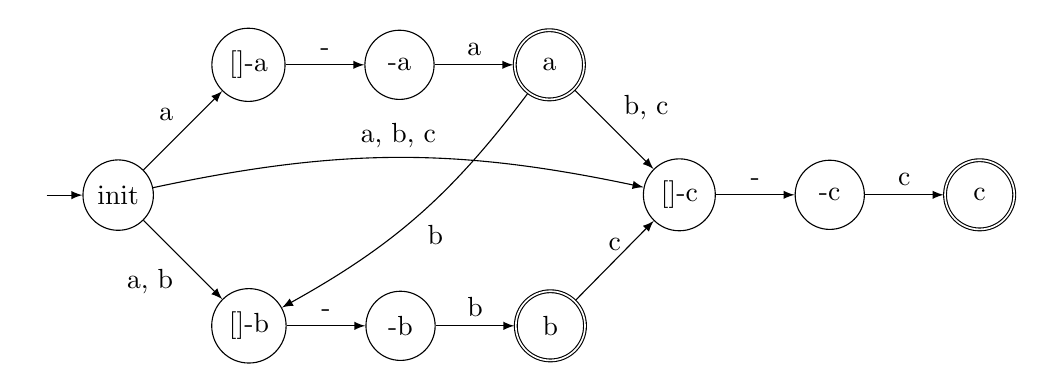
\begin{tikzpicture}[initial text={}, >={latex}]  
    \node[state, initial]   (0)                       {init};
    \node[state]            (a1) [above right=of 0]   {[]-a};
    \node[state]            (a2) [right=of a1]        {-a};
    \node[state, accepting] (a3) [right=of a2]        {a};
    \node[state]            (b1) [below right=of 0]   {[]-b};
    \node[state]            (b2) [right=of b1]        {-b};
    \node[state, accepting] (b3) [right=of b2]        {b};
    \node[state]            (c1) [below right=of a3]  {[]-c};
    \node[state]            (c2) [right=of c1]        {-c};
    \node[state, accepting] (c3) [right=of c2]        {c};
    
    \path[->] (0) edge                  node [above left]   {a}       (a1)
              (0) edge                  node [below left]   {a, b}    (b1)
              (0) edge  [bend left=12]  node [above]        {a, b, c} (c1)
              (a1) edge                 node [above]        {-}       (a2)
              (a2) edge                 node [above]        {a}       (a3)
              (a3) edge [bend left=12]  node [below right]  {b}       (b1)
              (a3) edge                 node [above right]  {b, c}    (c1)
              (b1) edge                 node [above]        {-}       (b2)
              (b2) edge                 node [above]        {b}       (b3)
              (b3) edge                 node [above]        {c}       (c1)
              (c1) edge                 node [above]        {-}       (c2)
              (c2) edge                 node [above]        {c}       (c3);
  \end{tikzpicture}
  \caption{The NFA generated using Algorithm \ref{alg:chars_inner} on the sorted alphabet $[a,b,c]$}
  \label{fig:chars_inner}
\end{figure}

Using an alphabet of size 10, we generated 784 regular expressions for each length in \{25, 50, 100, 150, 200, 300, 400, 500\}. This is sufficient for a 95\% confidence interval with a 3.5\% margin of error that our results are statistically correct. An alphabet of size 10 creates 10,945 inner character classes, and twice that many character classes when considering positive and negated versions.






\section{Implementing FAdo Extensions}
\label{sec:Implementing FAdo Extensions}
One of FAdo's main advantages is its extensibility. Main concepts such as regular expression tree nodes and NFAs are implemented as Python class objects, allowing each class to be extended with new features and functionality. Below is an overall view of how FAdo's classes were extended. The ``u'' prefix refers to forcibly using unicode symbols, and the ``Invariant'' NFA name is inspired as a non-transducer version of the automata from \cite{alphabet-invariant}.

\begin{multicols}{3}
  \begin{tabular}{l|l}
    FAdo class & Extension \\
    \hline
    regexp    & uregexp \\
    concat    & uconcat \\
    disj      & udisj \\
    star      & ustar \\
    option    & uoption \\
  \end{tabular}

  \begin{tabular}{l|l}
    FAdo class & Extension \\
    \hline
    epsilon   & uepsilon \\
    \empty    & anchor \\
    atom      & uatom \\
    \empty    & chars \\
    \empty    & dotany \\
  \end{tabular}
  
  \begin{tabular}{l|l}
    FAdo class & Extension \\
    \hline
    NFA       & InvariantNFA \\
  \end{tabular}
\end{multicols}


\subsection{Unicode Regular Expressions}
\label{subsec:Unicode Regular Expressions}
All regular expression classes have been extended to support the following features: partial derivative membership (Section \ref{sec:Derivatives}), pairwise language enumeration (Section \ref{subsec:Pairwise Word Generation}), backtracking word membership (Section \ref{sec:Backtracking Membership Algorithm}), explicit pointer-based tree compression (Section \ref{sec:Partial Derivative NFA}), partial matching anchor elimination construction (Section \ref{subsec:Partial Matching}), and displaying regular expression trees using graphviz \cite{graphviz}. And where relevant, FAdo bugs were fixed (e.g., \_delAttr not passing down to both children in concat class).

The following InvariantNFA constructions are supported: Thompson, Glushkov, position, follow, and partial derivative (through nfaPDO, nfaPDDAG, and nfaPDRPN). The nfaPDRPN (partial derivative reverse polish notation) construction was created as a further optimization of FAdo's optimized partial derivative NFA construction nfaPDO. The nfaPDO algorithm memoizes the linear form of regular expressions within each node in case the exact node needs its linear form again. Like with the naive nfaPD construction from Section \ref{sec:Partial Derivative NFA}, each NFA state is named according to its regular expression tree. Whenever a new transition is created in the NFA, the destination node is either created or found according to its name (recall: the state's name is a regular expression tree). Repeatedly comparing regular expression trees for equality is expensive. By contrast, the nfaPDRPN algorithm first compresses the regular expression tree \cite{pddag}, then names its NFA states with the RPN string of the regular expression tree. nfaPDRPN avoids the duplicate linear form function evaluations of nfaPDO, and speeds up NFA state lookup by naming states with strings rather than trees that have to be traversed for equality. The performance of this algorithm is explored in Chapter \ref{ch:Results}.

Additionally, all atomic subclasses (uatom, chars, and dotany) support taking the intersection with another atomic subclass. This is an important feature with respect to the product construction (Section \ref{sec:Product Construction}); especially with the added complexity of character classes. For the purpose of this thesis, the product construction is used for the cross-section language enumeration problem, and all comparisons are between an atom $\sigma$ and the wild dot. In this case, the intersection is simply $\sigma$.


\subsection{Regular Expression Tree Equality}
\label{subsec:Regular Expression Tree Equality}
The partial derivative membership and NFA construction algorithms make use of sets of distinct regular expressions to improve their performance. However, when a regular expression tree is directly added to a Python set object, the associated computational costs can become larger than expected. FAdo compares equality of two regular expression trees by first converting each tree into its \emph{repr} form, and then comparing the resulting strings. In Python, repr is an overridable instance method on every class object that returns a string representing that object; although not strictly required, repr should return the string that constructs the object being represented. In the case of a regular expression tree in FAdo, repr traverses the entire tree to create a string. For example:

\begin{center}
  \begin{tabular}{r l}
    Infix Syntax: & $a ((b + a) b^*)$ \\
    Repr Syntax:  & \texttt{concat(atom(a),concat(disj(atom(b),atom(a)),star(atom(b))))}
  \end{tabular}
\end{center}

Each time a regular expression tree is added to any set, its repr string is computed and saved internally within the set object. Now consider the definition of partial derivatives from Section \ref{sec:Derivatives}: each recursive step creates a new set, and when each regular expression tree is added, its repr string is linearly computed. Any algorithm that makes use of partial derivatives added directly to the set will experience these repeated linear cost repr computations.

This can be improved by saving the repr value for each subtree as it is computed the first time, and then referring back to this previously computed repr string. Instead of using sets of regular expression trees, use dictionaries of repr keys and tree values. When adding a regular expression to the dictionary, strings are directly compared for equality rather than having to traverse the entire tree again. For brevity, the RPN string was selected over the repr string in the implementation, but it serves the exact same purpose.

In the Results section, both pd and pdo represent partial derivative membership algorithms without constructing an NFA. The pd algorithm makes some use of string identification, while pdo (partial derivative optimized) makes use of string identification in a dictionary throughout the entire algorithm. A naive partial derivative algorithm using a set is far too unoptimized, and was not selected to be tested. Similarly, the partial derivative NFA can be constructed much more efficiently if the states of the NFA are identified by a string (nfaPDRPN) instead of a regular expression tree (nfaPDO).

\subsection{Invariant NFA}
Pure FAdo follows typical theory and implements its NFA transition function using single character string symbols. A HashMap uses an integer state index to find another HashMap of outgoing character transitions, and because this is an NFA, there can be multiple destinations given a single transition character.
\begin{center}
  HashMap$<$int, HashMap$<$character, Set$<$int$>>>$
\end{center}
This approach is extremely advantageous as finding the successors of a state given a symbol is a constant-time operation. So, evaluating NFA word membership of $w$ can be done in $O(n*|w|)$ time where $n$ is the number of states in the NFA.

However, in practice when using the large UTF-8 alphabet, creating individual transitions for every symbol in a character class or wild dot is extremely space inefficient. And although word evaluation is still fast with a good hash function, constructing the NFA in the first place becomes slow and impractical. Instead, in order to keep construction time reasonable, the InvariantNFA uses Python classes as its transitions (uatom, chars, and dotany). Like in pure FAdo, the string ``@epsilon'' represents the the empty string and Python class uepsilon; this allows more FAdo NFA methods to work without needing to be extended.
\begin{center}
  HashMap$<$int, HashMap$<T$, Set$<$int$>>>$ \\
  where $T \in \{\textrm{uatom}, \textrm{chars}, \textrm{dotany}, \textrm{``@epsilon''}\}$
\end{center}

The trade-off of this approach says that given a current state index and a symbol of the input word, each outgoing transition has to be matched individually. Although it could be expensive to analyze each outgoing transition for simple atomic membership, in practice there are relatively few outgoing transitions from an average state. Of the sampled practical regular expressions, no chosen NFA construction assigns an average state with more than 1.25 outgoing transitions (and the average number of transitions per state across all construction methods for the sampled practical regular expressions is approximately 1.187). Therefore it is straightforward to iterate through each outgoing transition as there is not generally a lot of them.





\section{Design of Experiments}
\label{sec:Design of Experiments}
There are three stages each regular expression must complete: (1) preparation, (2) construction into an appropriate form, and (3) word membership time. The untimed preparation stage generates an appropriate test-set of accepting and rejecting words using techniques from Section \ref{sec:Regular Language Enumeration}. Next, for each selected evaluation method we measure the time taken for the regular expression string to be parsed into a regular expression tree that allows partial matching, then potentially converted into an InvariantNFA. Finally, we measure the time it takes this final structure to decide membership of all the accepting and rejecting words. No membership test is allowed to save any information to be used on a later membership test. In real implementations, it may be beneficial to save certain information (like previously computed partial derivatives), but this hurts our ability to fairly scale the number of word evaluations. It may be beneficial to build a more expensive NFA (like the partial derivative NFA) if you are evaluating thousands of words, while if you only evaluate one word another approach may be optimal. Our methods will retain the ability to contrast these algorithms with different capacities of input words.

We considered three membership algorithms that can be applied directly on the regular expression tree: word derivatives, partial derivatives, and backtracking. In each case, the construction stage does not need to build an InvariantNFA. Word derivatives ($D_\sigma$ function from Section \ref{sec:Derivatives}) were initially tested, but due to their exponential blow-up during membership evaluation it became obvious practical implementations should avoid this method. A naive partial derivative algorithm directly inserts the partial derivatives of a regular expression into a set, but the chosen implementation is more efficient because it uses string equality instead of tree equality (Section \ref{subsec:Regular Expression Tree Equality}). The pd algorithm uses string key identification within the membership method only, and the pdo algorithm uses this approach both in the membership and recursive partial derivative methods. Unfortunately, the pdo optimization was conceived at a late stage of the thesis and there was only enough time to test the pdo algorithm on practical regular expressions. Finally, because most practical regular expression libraries support backreferences and therefore use backtracking membership, we wanted to test this approach in our framework.

Another approach to solving word membership is to build an InvariantNFA, and then run the standard membership algorithm on it. FAdo's implementations of Thompson, Glushkov, position, follow ($\epsilon$-free), and a few partial derivative constructions were extended to create uatom, chars, dotany, and ``@epsilon'' transitions. The non-optimized partial derivative automaton construction (nfaPD) was not selected since a superior algorithm already exists within FAdo: nfaPDO. The optimized partial derivative NFA construction uses memoization and is much faster. Two additional partial derivative constructions were also selected: nfaPDDAG and nfaPDRPN.

The above process was completed independently for both practically sampled and randomly generated regular expressions. Separating random and practical expressions allows the analysis to compare the results from each sample. For each evaluation method, we create a plot using every regular expression. This plot compares the time to accept or reject the average tested word against the tree length of the regular expression. The time measurement considers the construction time $n$ times and the average word evaluation $m$ times. Additionally, to smooth the plot we group regular expressions into bins according to their tree length; this bin size is also configurable.

The main tests were conducted on a virtual private server (VPS) from Microsoft Azure (B4ms). This VPS was configured with 16 GB of memory and 4 virtual CPU cores. Up to 4 tests were computed in parallel; this number would shrink if there was a memory bottleneck, because sometimes the generated test set of words required several GB of memory (particularly with large randomly generated regular expressions with nested star operations), and we want to avoid using slow memory swap onto the disk. Each CPU-bound test process was given a ``nice value'' of -20, meaning the process scheduler would prioritize these processes above all others. The built-in Python module timeit was selected to measure the relevant times; it chooses the most precise time implementation for the system, and ensures garbage collection is turned off. If we were using Python $>3.3$, we would use time.process\_time() to measure CPU time directly. 

An indicator of the efficiency of a regular expression's NFA is the number of states plus the number of transitions. For every practically sampled regular expression and supported NFA construction method we save the resulting NFA in a database \cite{dill} along with the number of states and the number of transitions. This analysis is completed to show how various NFA constructions scale on a practical sample of regular expressions. Although time measurements were taken, they were not the focus of this analysis, and therefore this was the only test executed on a personal computer.




























  
  \chapter{Results}
  \label{ch:Results}
  First, we analyze the size of the tested NFA constructions on the sample of practical regular expressions. There were four resulting NFAs constructed: Thompson, Glushkov, follow, and the partial derivative NFA. The position construction creates an identical NFA to Glushkov, and the partial derivative NFA has been constructed using nfaPDO, nfaPDRPN, and nfaPDDAG methods. Secondly, we analyze the performance of each membership evaluation algorithm independently on practical and randomly generated regular expressions. Membership is tested on each of the seven NFA constructions using the standard NFA membership algorithm that tracks a set of current states as each symbol of the input word is consumed. Additionally, three non-NFA methods were tested: backtracking, partial derivatives (pd), and optimized partial derivatives (pdo). Table \ref{tbl:Summary of algorithms} shows a summary of the tested methods below. The pdo algorithm was created too late into this thesis to test on randomly generated regular expressions, and the backtracking algorithm frequently experienced exponential membership time for the random sample, so neither of these methods were completed for the randomly generated sample.

\begin{table}[H]
  \doublespacing
  \centering
  \begin{tabular}{l| |c c l}
                & \multicolumn{2}{c}{Expression Type} \\
    Algorithm   & Practical & Random & Description \\
    \hline
    \hline
    Thompson    & Yes & Yes & Thompson construction \\
    Glushkov    & Yes & Yes & Glushkov construction \\
    Position    & Yes & Yes & Position construction \\
    Follow      & Yes & Yes & $\epsilon$-free follow construction \\
    PDO         & Yes & Yes & Optimized partial derivative construction \\
    PDRPN       & Yes & Yes & Partial derivative construction with string keys \\
    PDDAG       & Yes & Yes & Partial derivative construction using a DAG \\
    \hline
    pd          & Yes & Yes & Partial derivatives (non-NFA) \\
    pdo         & Yes & No  & Partial derivatives (non-NFA) with string keys \\
    backtrack   & Yes & No  & Exponential backtracking
  \end{tabular}
  \caption{Summary of tested algorithms}
  \label{tbl:Summary of algorithms}
\end{table}


\section{NFA Sizes for Practical Regular Expressions}
\label{sec:NFA Sizes for Practical Regular Expressions}
An indication of an NFA's efficiency is its size. So, given practically sampled regular expressions, how large are the resulting NFAs by their regular expression tree length? We have $12,023$ unique practical regular expressions, each with two forms: partial matching and non-partial matching. Since partial matching regular expression $\alpha$ might be equivalent to non-partial matching regular expression $\beta$ ($\alpha \neq \beta$), only one of $\alpha, \beta$ is kept. After considering this, we have $23,253$ unique regular expressions. If any construction takes longer than two minutes, it is preempted and thrown away. Table \ref{tbl:nfa sizes} shows that the PDO method is the most limiting factor for these constructions, and as such we have $23,247$ regular expressions that are successful for all construction methods. This table also shows the amount of time it took to construct the regular expressions into NFAs, but this measurement should be taken \emph{very lightly} since the number of regular expressions for each method may be unequal, and that it was performed on a personal computer instead of a server.

\begin{table}[H]
  \center
  \begin{tabular}{l|c|c}
    Method & \# Regular Expressions & Time taken (s) \\
    \hline
    Follow     & 23,253 & 26.968 \\
    Glushkov   & 23,253 & 36.084 \\
    Position   & 23,253 & 38.332 \\
    PDDAG      & 23,253 & 73.251 \\
    Thompson   & 23,251 & 141.28 \\
    PDRPN      & 23,251 & 260.19 \\
    PDO        & 23,247 & 680.46 \\
  \end{tabular}
  \caption{The number of regular expressions constructed by method without preemption}
  \label{tbl:nfa sizes}
\end{table}

Figure \ref{fig:nfa_sizes} plots the sizes of different NFAs for all $23,247$ non pre-empted regular expressions common to every construction method. We correctly assert that PDO, PDDAG, and PDRPN all construct the same partial derivative NFA; as well, the Glushkov and position constructions build an identical NFA. Partial derivative constructions create the smallest NFA, then the follow construction, position/Glushkov, and finally the Thompson NFA.

\begin{figure}[H]
  \center
  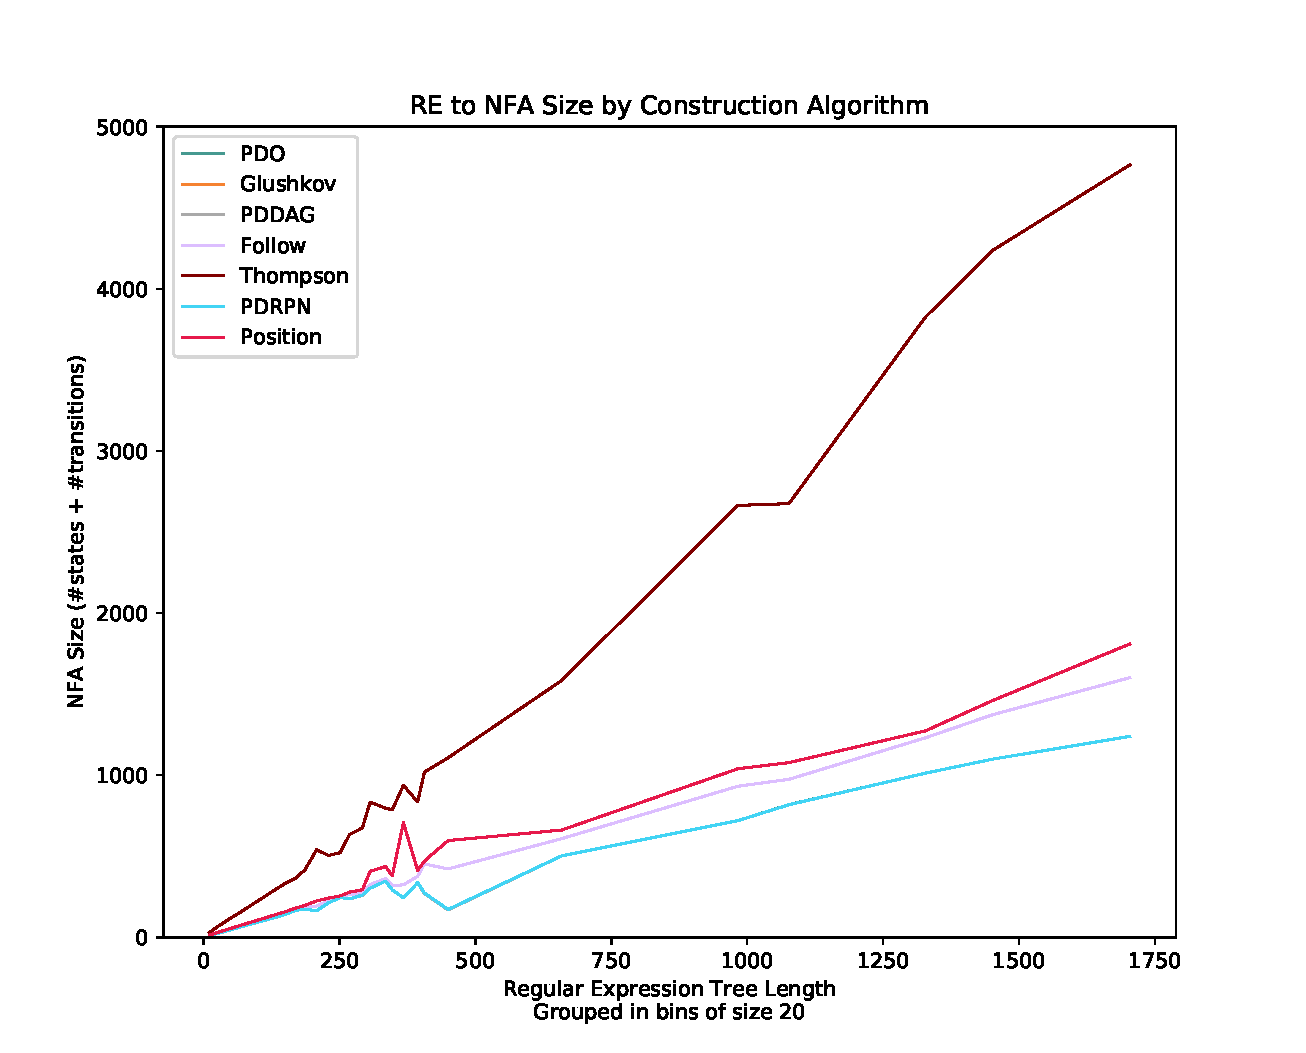
\includegraphics[width=0.75\linewidth]{fig/nfa_sizes}
  \caption{Sizes of the NFAs produced using different construction methods and practical regular expressions}
  \label{fig:nfa_sizes}
\end{figure}





\section{Practical Regular Expressions}
\label{sec:Practical Regular Expressions}
We found 12,023 unique regular expressions that could be successfully converted into their equivalent mathematical syntax. Due to time constraints, only 10,686 regular expressions have been fully tested using each method. Table \ref{tbl:practical sample by tree length} shows the distribution of the sampled practical regular expressions by their tree length, and the quantity that have been fully tested. Beyond tree length 175, we only have single-digit quantities and we are therefore not confident to make any conclusions; all plots of measuring the performance of practical regular expressions will only include regular expressions with tree length less than 180 (of which we have  $\approx$10,662, depending on the unimportant distribution within $[175, 200)$).

\begin{table}[H]
  \center
  \begin{tabular}{c|c|c}
    Tree Length & \# Expressions & \# Completed \\
    \hline
    $[0, 25)$     & 8,053 & 7,185 \\
    $[25, 50)$    & 2,560 & 2,305 \\
    $[50, 75)$    & 832   & 747 \\
    $[75, 100)$   & 272   & 239 \\
    $[100, 125)$  & 136   & 98 \\
    $[125, 150)$  & 79    & 55 \\
    $[150, 175)$  & 49    & 30 \\
    $[175, 200)$  & 10    & 3
    % Total:        11,991  10,662
  \end{tabular}
  \caption{The number of practical regular expressions by tree length}
  \label{tbl:practical sample by tree length}
\end{table}

\begin{figure}[H]
  \center
  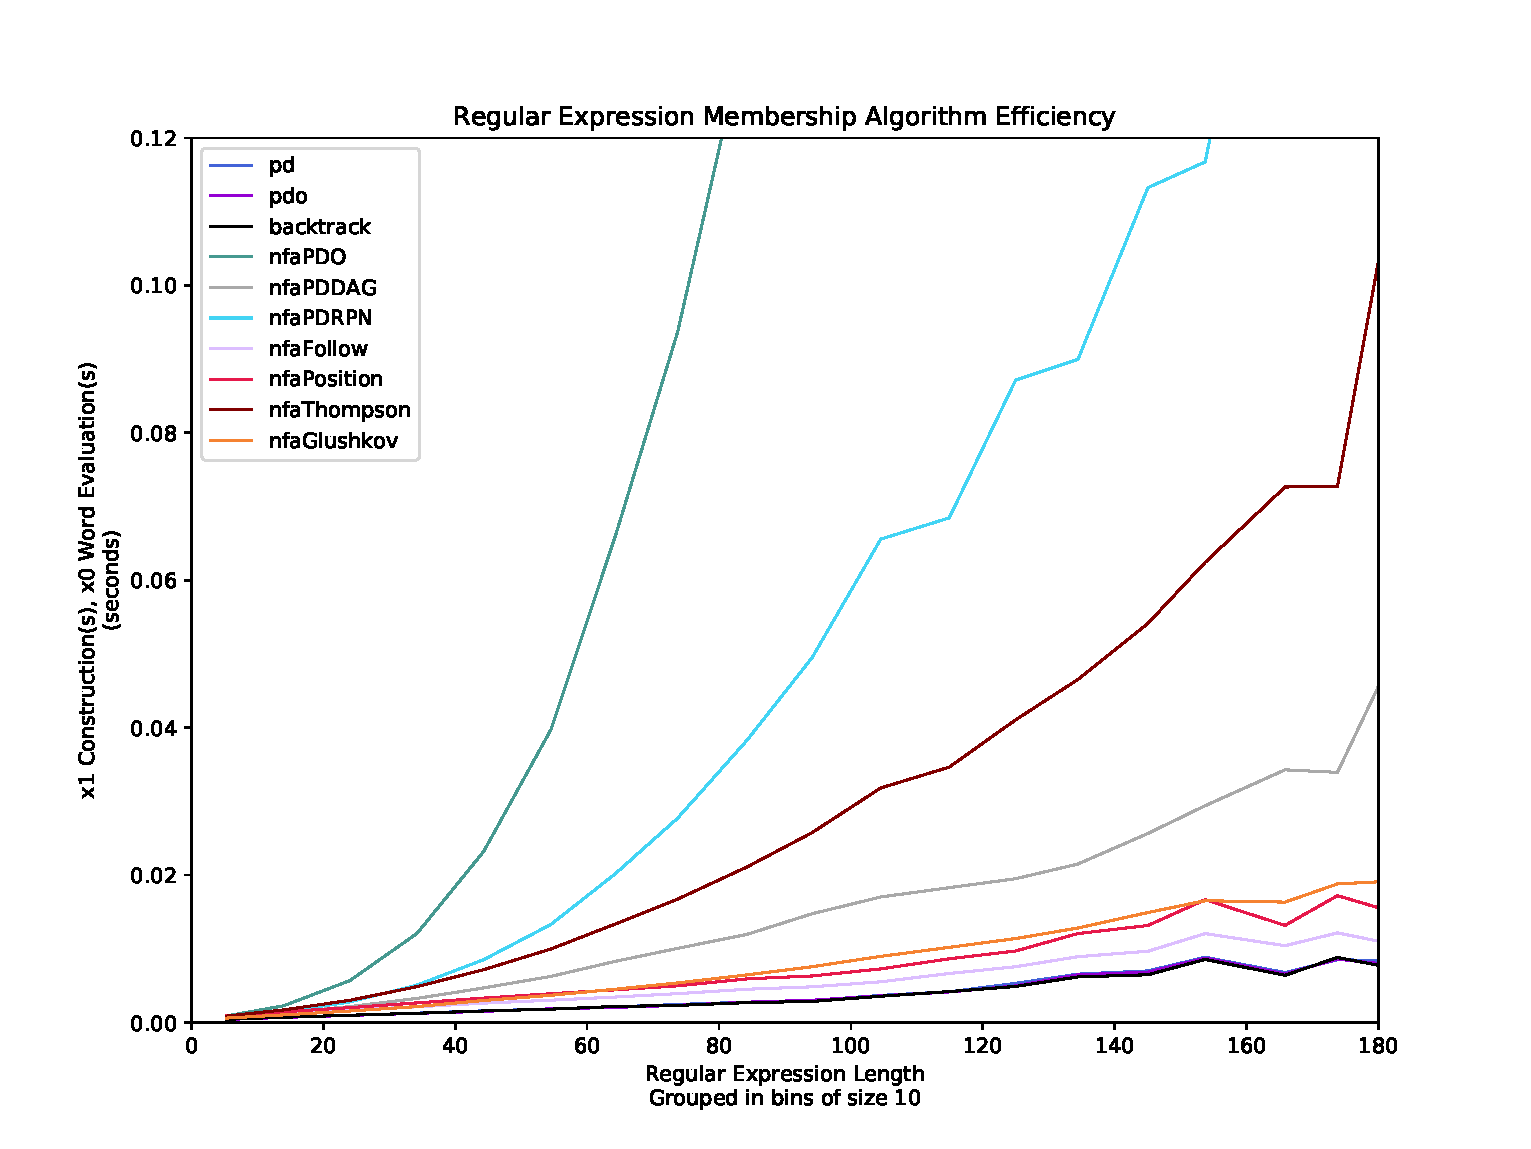
\includegraphics[width=0.75\linewidth]{fig/prac/1construction}
  \caption{Construction time by method for practical regular expressions}
  \label{fig:prac/1construction}
\end{figure}

Figure \ref{fig:prac/1construction} shows the time taken to construct an appropriate Python class object starting at a mathematical regular expression string. As expected, the methods which do not construct an NFA represent the fastest constructions (pd, pdo, and backtrack all have an identical construction into a partial matching regular expression tree). The remaining NFA constructing methods are given in increasing order: follow, position, Glushkov, nfaPDDAG, Thompson, nfaPDRPN, and finally nfaPDO.

Once the structure is constructed, we must consider the efficiency of the different membership algorithms. Figure \ref{fig:prac/1evaluation} compares the different methods. Both non-NFA partial derivative algorithms (pd and pdo) are significantly slower to evaluate word membership than all other tested methods. The backtracking algorithm is frequently the fastest, but occasionally experiences spikes where excessive backtracking was required. The NFAs are divided into two classes according to membership time: sequential NFAs (PDO/PDRPN/PDDAG, Glushkov/position, and follow), and the Thompson NFA with $\epsilon$-transitions. These empty transitions delay word matching and therefore result in a slower membership process. In reality, the backtracking algorithm occasionally failed all together when Python's maximum recursion depth (set to 12,000) was exceeded. Presumably, this issue could be solved by refactoring the backtracking algorithm to use an iterative approach, so any time the maximum recursion depth was reached, the regular expression was removed from our results set for every method.

\begin{figure}[H]
  \centering
  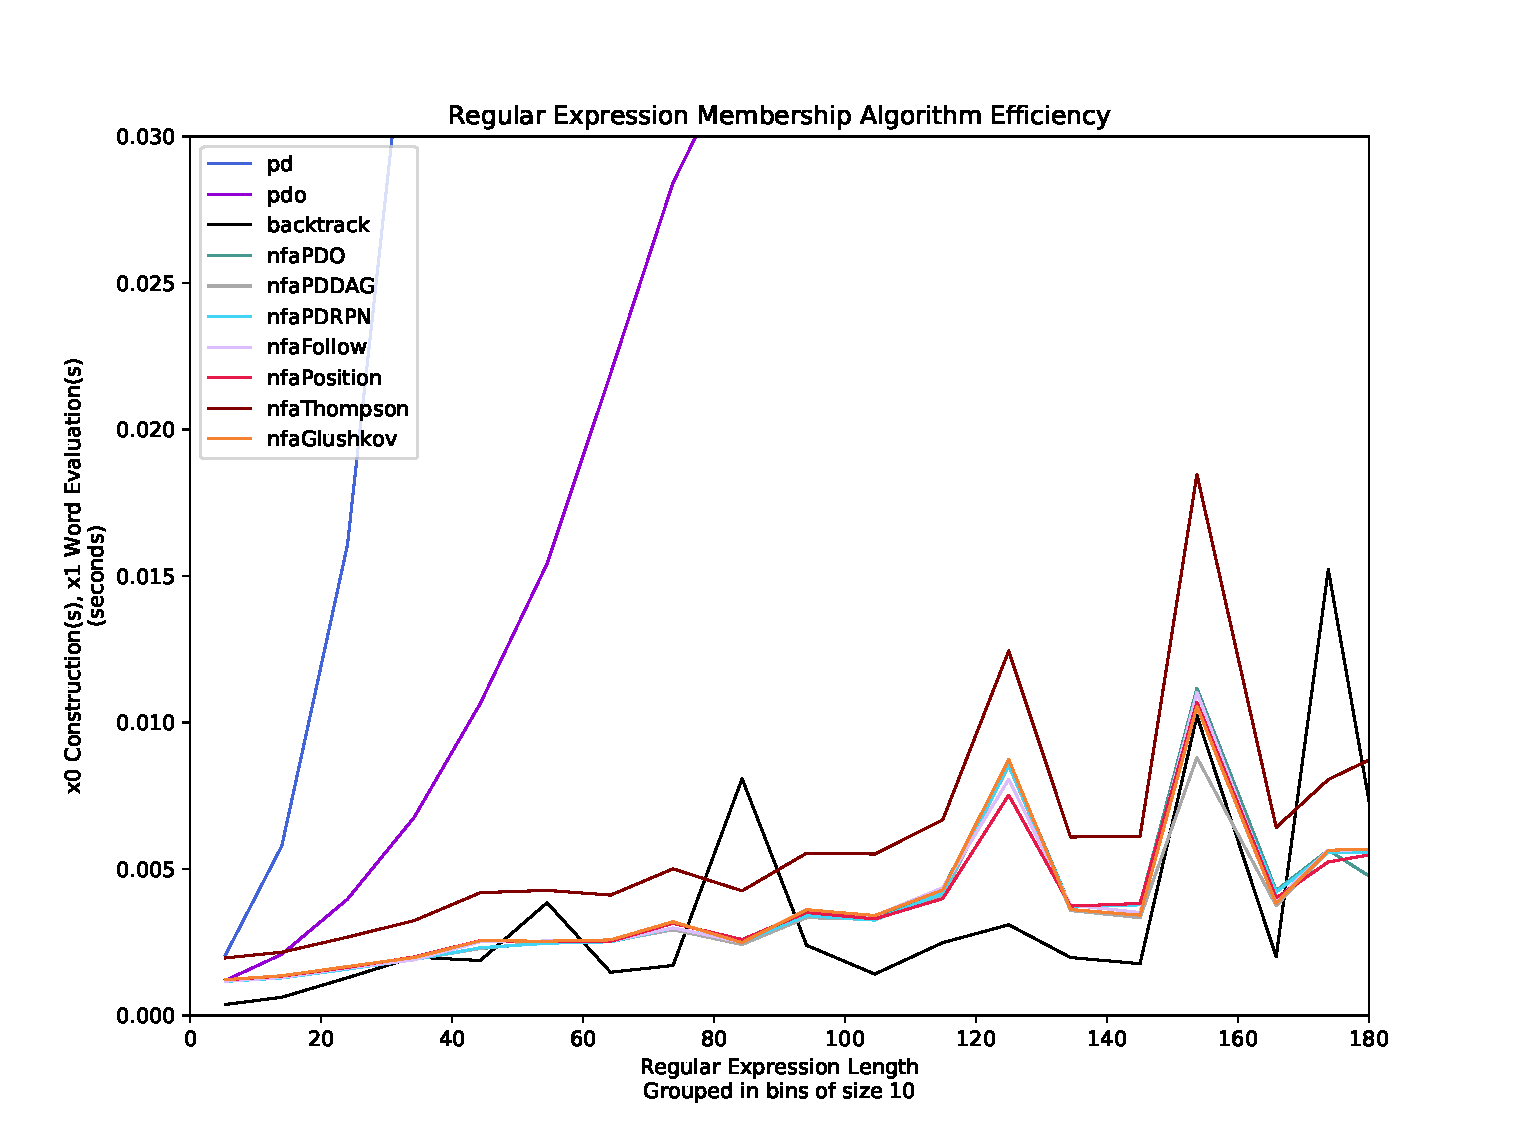
\includegraphics[width=0.75\linewidth]{fig/prac/1evaluation}
  \caption{Word membership time of practical regular expressions after construction has taken place}
  \label{fig:prac/1evaluation}
\end{figure}

Often, regular expressions are used to evaluate the membership of just a single input word. In this case, Figure \ref{fig:prac/1const1eval} compares solutions to the one-word membership problem using each of our algorithms. The backtracking algorithm continues to be impressively fast, due to its low construction cost and average fast membership time. The follow algorithm has a small edge over nearly equivalent position and Glushkov constructions. Then, with larger time gaps: nfaPDDAG, Thompson, pdo, nfaPDRPN, nfaPDO, and finally pd. This is very similar to Figure \ref{fig:prac/1construction} since word membership takes far less time on average than construction time.

\begin{figure}[H]
  \center
  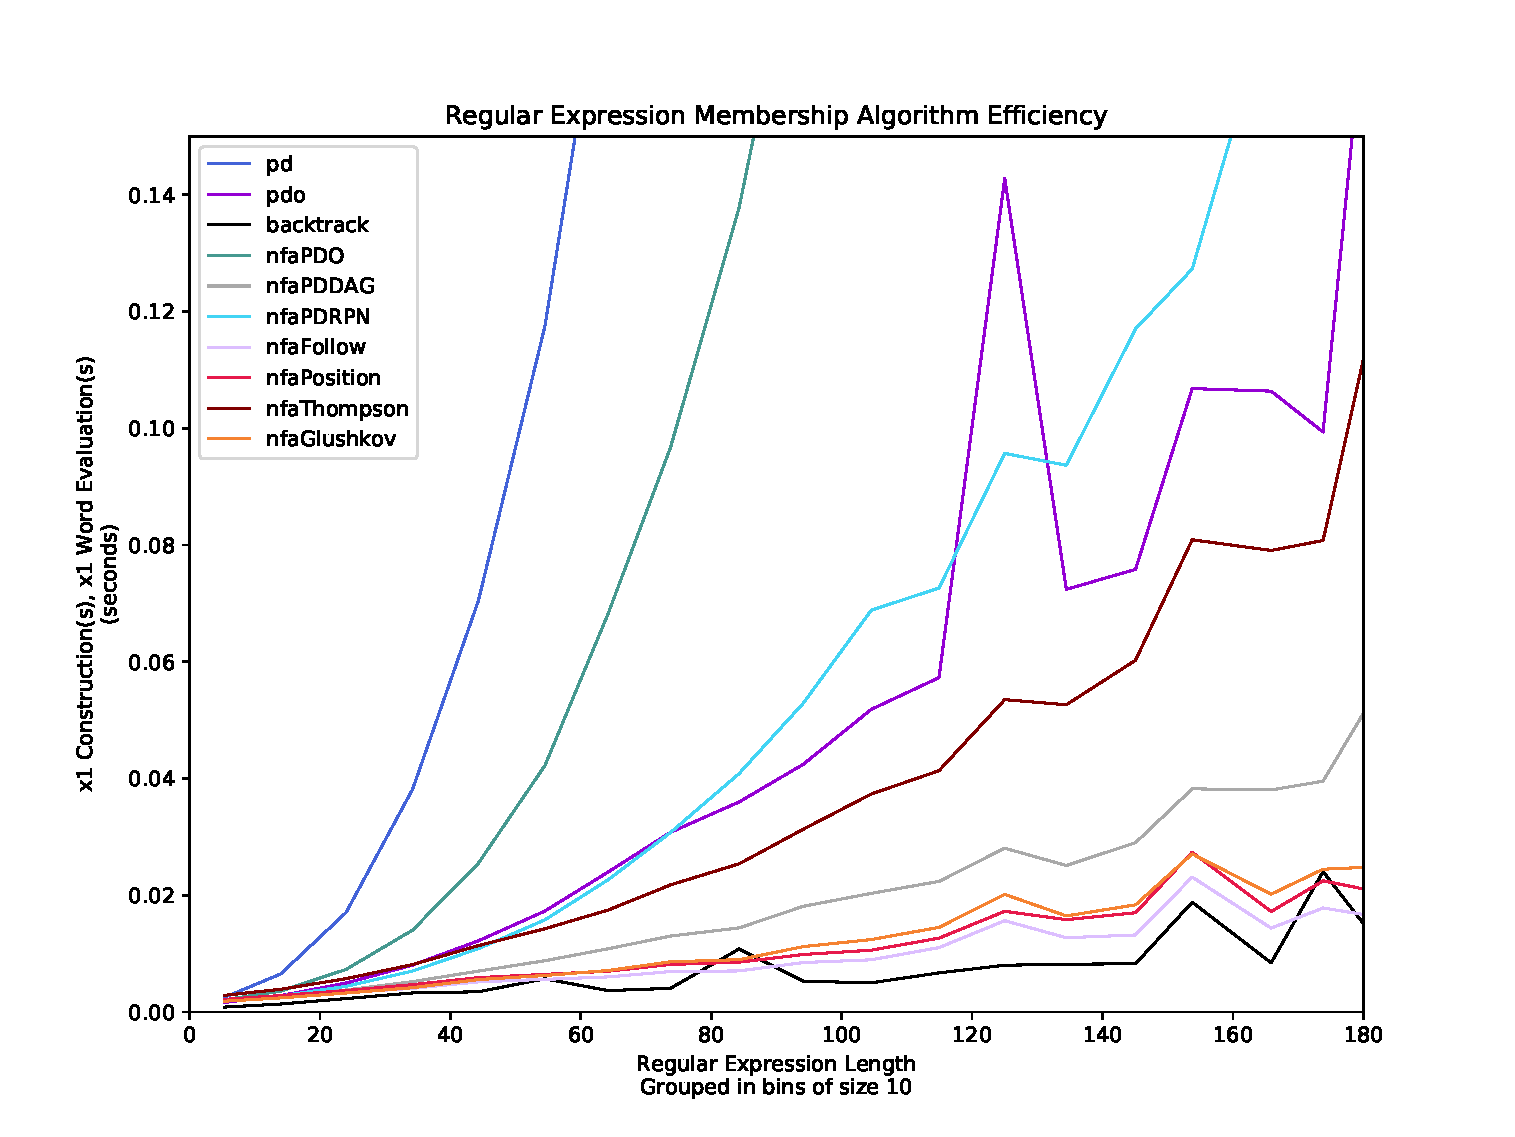
\includegraphics[width=0.75\linewidth]{fig/prac/1const1eval}
  \caption{Sum of construction time and one-word membership time for practical regular expressions}
  \label{fig:prac/1const1eval}
\end{figure}

A key observation from Figure \ref{fig:prac/1const1eval} is the pdo algorithm is faster on average than the nfaPDO and nfaPDRPN methods. The partial derivative NFA is constructed by considering \emph{every} possible partial derivative with respect to \emph{every} alphabet symbol, but the (non-NFA) partial derivative algorithm only computes the partial derivatives with respect to the specific input word. Equivalently, only a subset of the states in the partial derivative NFA are useful for the computation for a given input word; so the overall computation cost can be mitigated by only constructing the useful states. The pdo algorithm is based on the same methodology as the nfaPDRPN construction, and it makes sense that pdo is faster when considering a single input word. Using nfaPDDAG as inspiration, there should be a (non-NFA) partial derivative algorithm which computes membership faster than PDDAG can be constructed and membership evaluated; but to our knowledge no such algorithm currently exists.

Perhaps the regular expression is used to filter data from a database with 100,000 records. Figure \ref{fig:prac/1const10e6eval}(a) shows that as long as the regular expression library is using a sequential NFA to decide membership, there is little relative difference between construction algorithms. With so many word evaluations, even the slow nfaPDO construction is acceptable. Because the overall time is dominated by word membership tests, the construction time is unimportant. NFAs compute all possible paths through the regular expression at construction-time, whereas pd, pdo, and backtrack algorithms do this at membership-time. The pd and pdo algorithms are blown away, but backtracking remains generally competitive assuming the expression is not vulnerable to catastrophic backtracking. Like in Figure \ref{fig:prac/1evaluation}, the sequential NFAs provide an advantage over the Thompson NFA. It is difficult to declare a clear winner among the sequential NFA methods, but Figure \ref{fig:prac/1const10e6eval}(b) attempts to do so by decreasing the resolution (using more averaging) and zooming into a focused region. The nfaPDDAG algorithm is the fastest, followed by the other partial derivative NFAs, and then nearly equivalent Glushkov, position, and follow NFA methods. 

\begin{figure}[H]
  \centering
  \begin{subfigure}[b]{0.45\linewidth}
    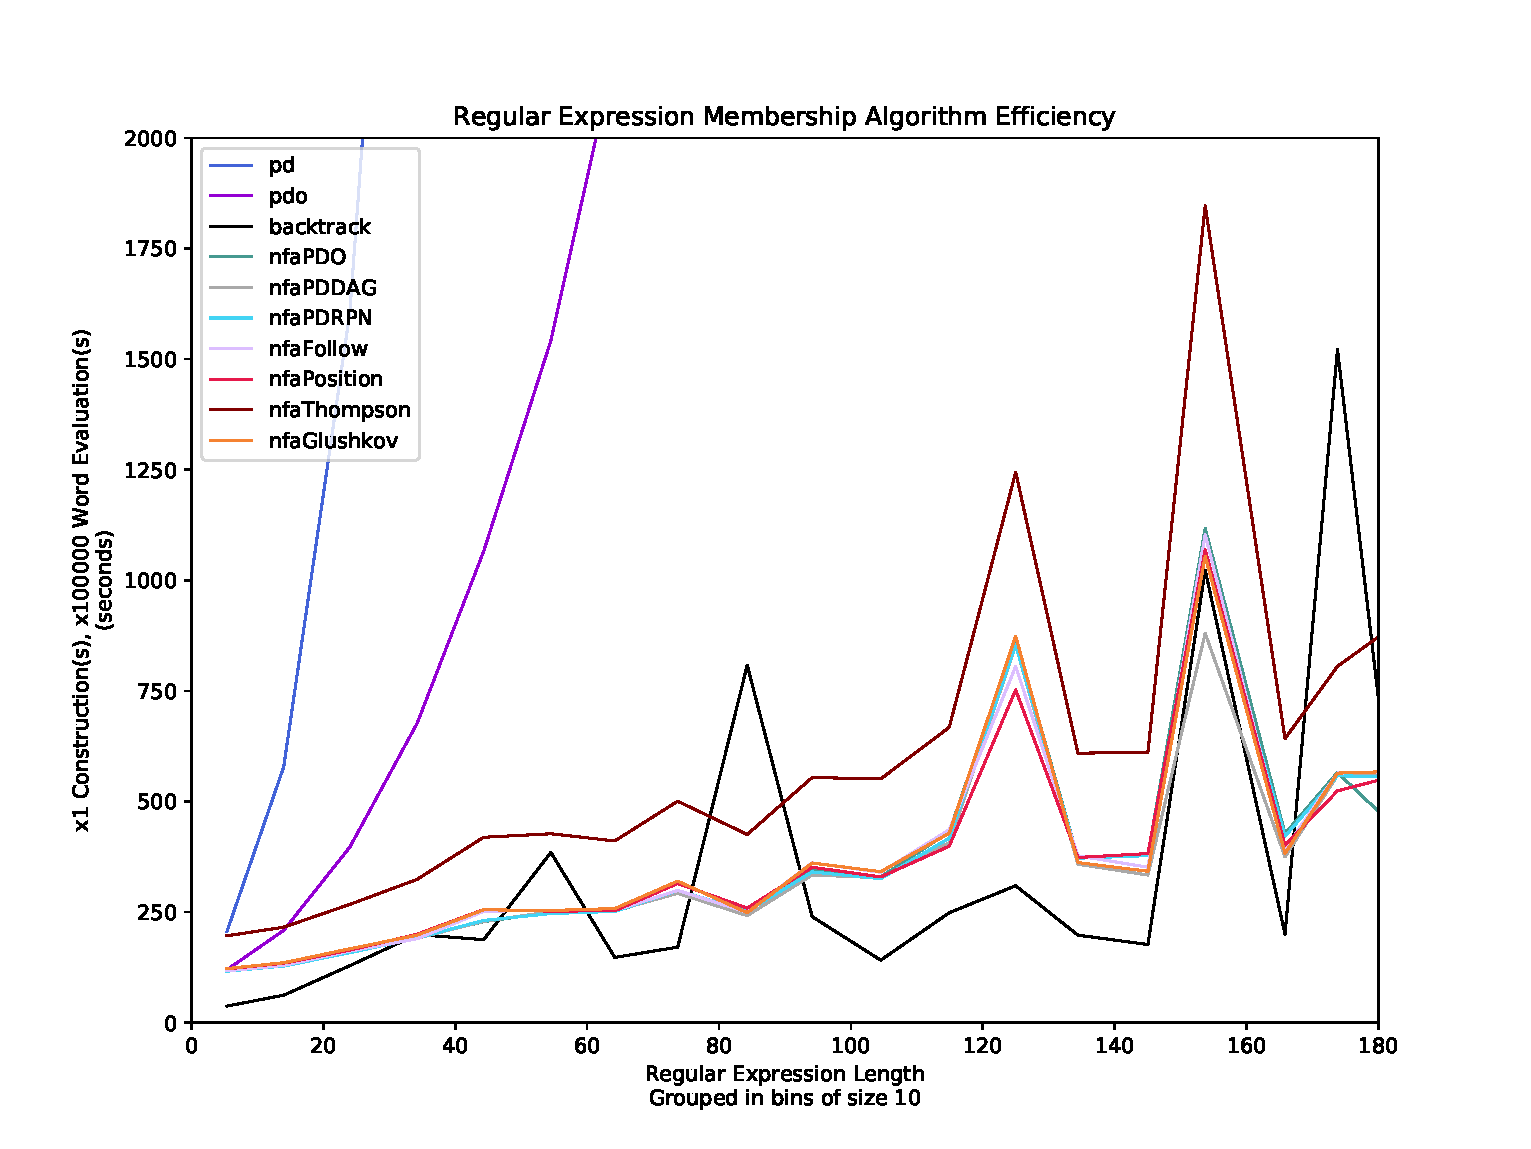
\includegraphics[width=\linewidth]{fig/prac/1const10e6eval}
    \caption{Full picture: length bins of tree length 10}
  \end{subfigure}
  \begin{subfigure}[b]{0.45\linewidth}
    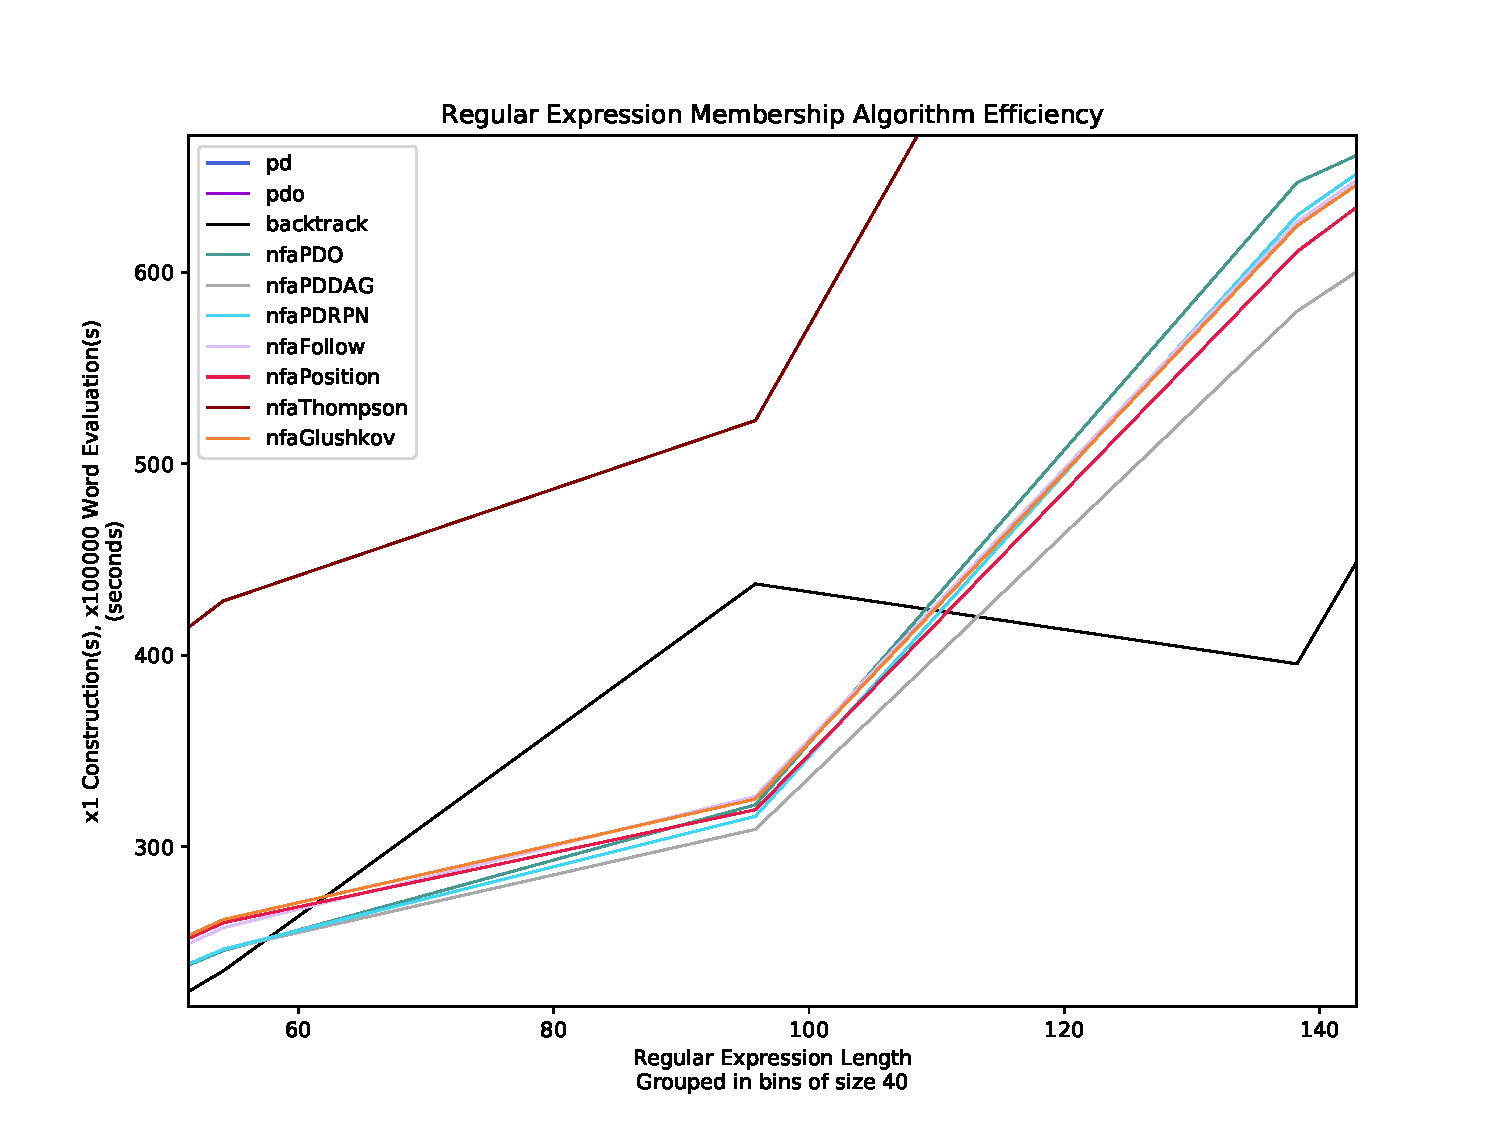
\includegraphics[width=\linewidth]{fig/prac/1const10e6eval_zoomed}
    \caption{Zoomed in: length bins of tree length 40}
  \end{subfigure}
  
  \caption{Sum of construction time and 100,000 word membership time for practical regular expressions}
  \label{fig:prac/1const10e6eval}
\end{figure}





\section{Randomly Sampled Regular Expressions}
\label{sec:Randomly Sampled Regular Expressions}
Using the same testing framework for randomly generated regular expressions allows us to compare the results with practical expressions. It also gives us more control and confidence: 784 regular expressions with alphabet of size $10$ were generated for each tree length \{25, 50, 100, 150, 200, 300, 400, 500\}. We were unable to sample many practical regular expressions beyond tree length 200, so this will give a much better picture how these algorithms perform for longer expressions. Once the tests are complete, we have a 95\% confidence interval with a 3.5\% margin of error. However once again, the test set is incomplete due to both time constraints and memory issues related to deeply nested star operations and pairwise (Section \ref{subsec:Pairwise Word Generation}) language generation within the set of randomly generated regular expressions. Table \ref{tbl:random sample by tree length} shows the amount each tree length has been completed. Instead, we are 95\% confident that our results are statistically correct with a margin of error no more than 5\% for all tree lengths except 500.

\begin{table}[H]
  \center
  \begin{tabular}{c|c|c}
    Tree Length & \# Expressions & \# Completed \\
    \hline
    $25$    & 784 & 783 \\
    $50$    & 784 & 780 \\
    $100$   & 784 & 769 \\
    $150$   & 784 & 741 \\
    $200$   & 784 & 688 \\
    $300$   & 784 & 581 \\
    $400$   & 784 & 422 \\
    $500$   & 784 & 286
    % Total:  6,272 5,050
  \end{tabular}
  \caption{The number of randomly generated regular expressions by tree length}
  \label{tbl:random sample by tree length}
\end{table}

The backtracking membership algorithm frequently experienced exponential membership time for randomly generated regular expressions. There are a few reasons why this could make sense: (1) programmers may be aware of catastrophic membership and therefore write their regular expressions to not be vulnerable, (2) vulnerable regular expressions may not be useful for GitHub developers, or (3) a small alphabet with nested star operations allow input words to be matched in complex ways. Because the backtracking algorithm was taking too long, it was disabled so the rest of the tests could be run in our lifetimes. In addition, the results for the pdo algorithm were not completed for the randomly generated set of regular expressions because the pdo algorithm was created only recently.

\begin{figure}[H]
  \center
  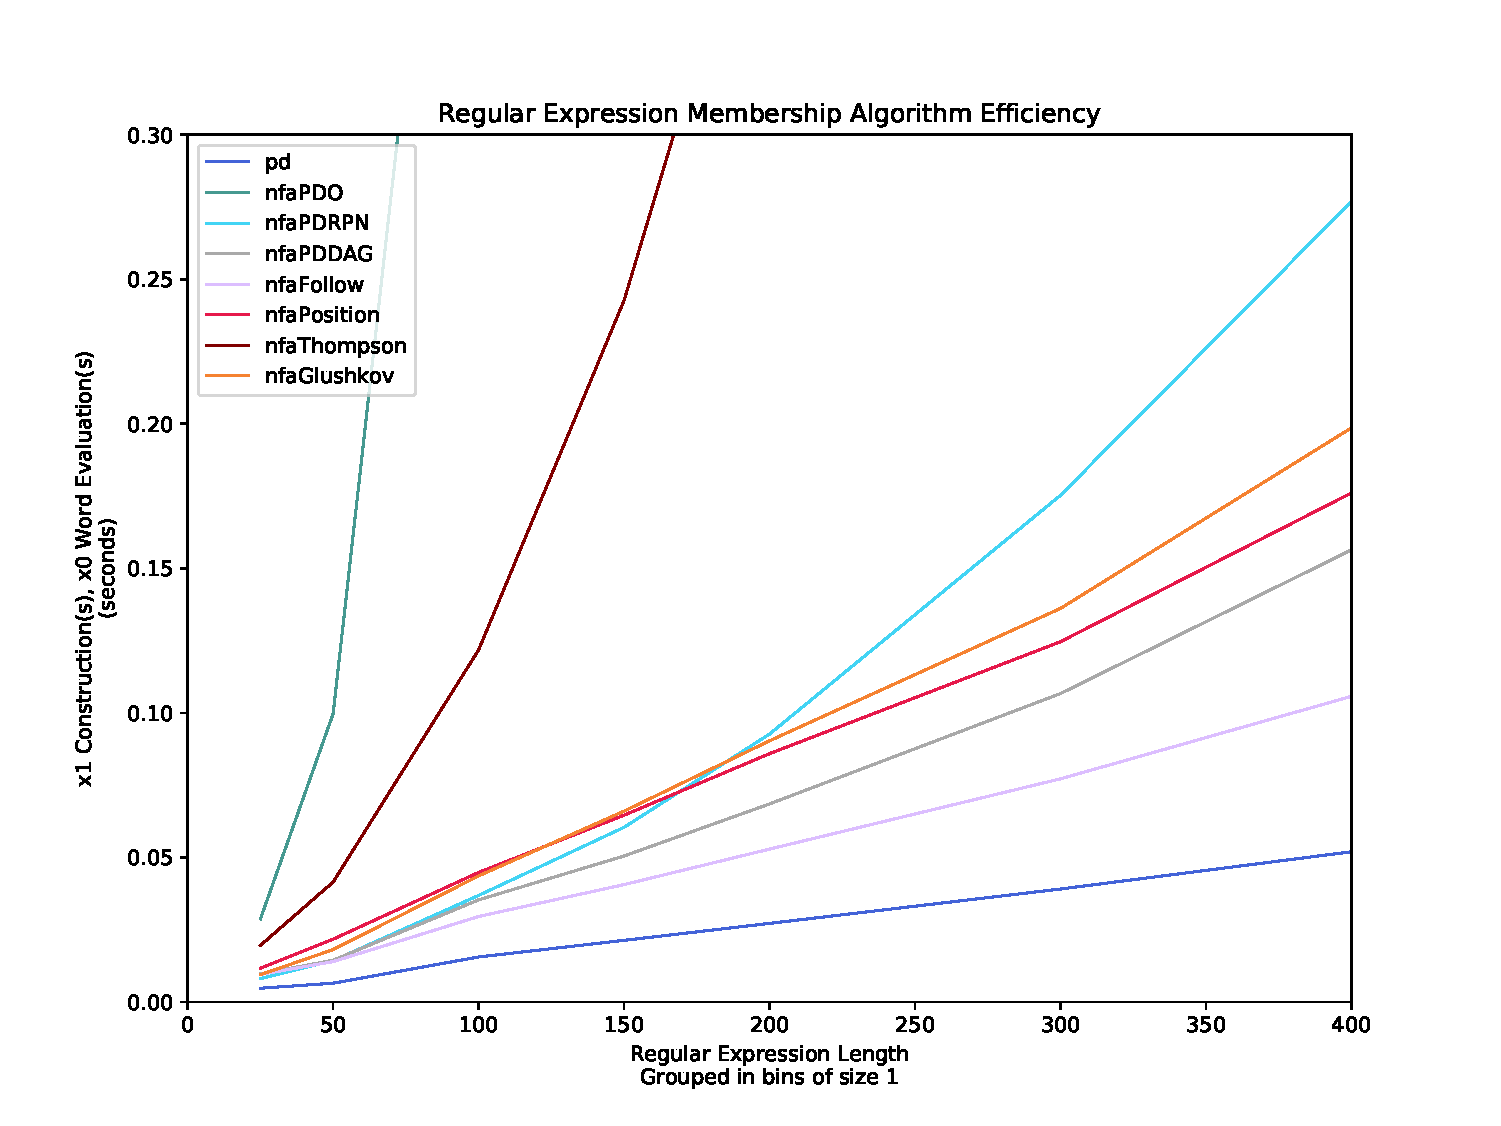
\includegraphics[width=0.75\linewidth]{fig/rand/1construction}
  \caption{Construction time by method for randomly generated regular expressions}
  \label{fig:rand/1construction}
\end{figure}

Figure \ref{fig:rand/1construction} shows the construction times for each of the algorithms. Once again the pd algorithm has the least construction time because it does not construct an NFA, and the nfaPDO and Thompson algorithms are very slow. All other sequential NFA constructions are given by increasing speed: follow, nfaPDDAG, position, Glushkov, and finally nfaPDRPN. It is exciting to see the nfaPDDAG algorithm performing so well; since the partial derivative NFA was previously so far out of reach with the nfaPDO method.

In Figure \ref{fig:rand/1evaluation} we get a look at word membership times. The time scale is significantly larger than with practical regular expressions because the accepted words are sometimes extremely long using the modified combination generation approach with deeply nested stars. However, the relative ranking of each method is still comparable because the exact same input words are generated for any given regular expression. The Thompson NFA continues to have $\epsilon$-transitions that delay word matching, and is therefore the slowest. Each of the partial derivative NFAs are very close (as they should be, since they generate the same NFA). The position algorithm appears to be slightly faster than follow, which is slightly faster than Glushkov. Remarkably for much of the domain, the (non-NFA) partial derivative algorithm is the fastest. And we would expect the pdo algorithm to speed up this computation even more. This is in direct contrast to practical regular expressions where the partial derivative algorithm is the slowest. Why are partial derivatives so much better in randomly generated regular expressions?

\begin{figure}[H]
  \center
  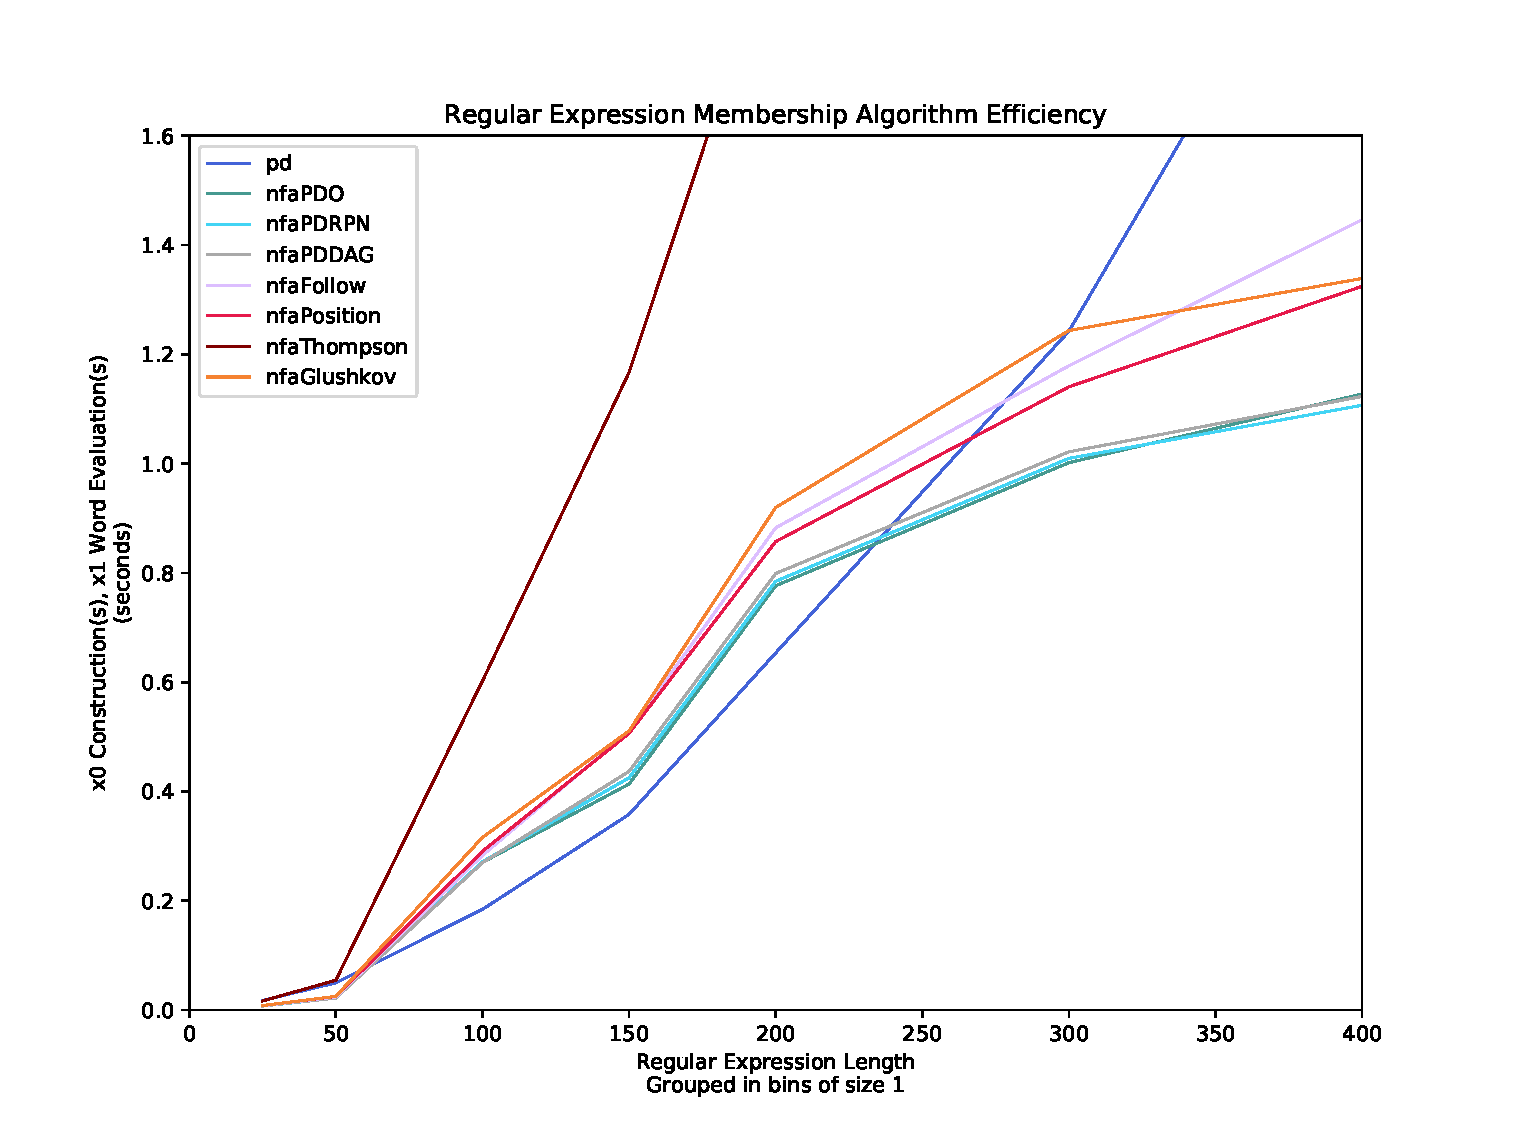
\includegraphics[width=0.75\linewidth]{fig/rand/1evaluation}
  \caption{Word membership time of randomly generated regular expressions after construction has taken place}
  \label{fig:rand/1evaluation}
\end{figure}

An analysis of the composition of practical and randomly generated regular expressions exposes a potential answer. Since membership is tested on regular expressions with partial matching enabled, this analysis first enabled partial matching on each expression before checking the relative frequency of internal nodes. Recall: optional operations are removed in favour for a disjunction with the empty word in the anchor elimination construction.

\begin{table}[H]
  \centering
  \begin{tabular}{r|c c}
    \empty & Practical Expressions & Random Expressions \\
    \hline
    Concatenation & $78.99\%$ & $43.02\%$ \\
    Disjunction   & $3.10\%$  & $41.93\%$ \\
    Star          & $17.91\%$ & $15.05\%$
  \end{tabular}
  \caption{Relative frequencies of internal nodes in the regular expression samples}
  \label{tbl:composition}
\end{table}

As shown in Table \ref{tbl:composition}, practically sampled regular expressions have almost twice as many concatenations as randomly generated expressions. Recall the partial derivative definition for concatenation from Section \ref{sec:Derivatives}:
\begin{center}
  $$
  \delta_\sigma(\alpha \beta) = \begin{cases}
    \delta_\sigma(\alpha)\{\beta\}                            & \epsilon \notin L(\alpha) \\
    \delta_\sigma(\alpha)\{\beta\} \cup \delta_\sigma(\beta)  & \epsilon \in L(\alpha)
  \end{cases}
  $$
\end{center}
Calculating the partial derivative set of a concatenation requires checking if the empty word is accepted by the left child ($\alpha$). Consider converting the programmer's regular expression $a\{6\}$ into the mathematical regular expression using methods from Section \ref{subsec:Converting into FAdo Compatible Syntax}. The tree in Figure \ref{fig:left vs right expansion}(a) is the result.
\begin{figure}[H]
  \centering
  \begin{subfigure}[b]{0.45\linewidth}
    \centering
    \Tree
    [
      .$\odot$
      [
        .$\odot$
        [
          .$\odot$
          [
            .$\odot$
            [
              .$\odot$
              a
              a
            ]
            a
          ]
          a
        ]
        a
      ]
      a
    ]
    \caption{Left expansion}
  \end{subfigure}
  \begin{subfigure}[b]{0.45\linewidth}
    \centering
    \Tree
    [
      .$\odot$
      a
      [
        .$\odot$
        a
        [
          .$\odot$
          a
          [
            .$\odot$
            a
            [
              .$\odot$
              a
              a
            ]
          ]
        ]
      ]
    ]
    \caption{Right expansion}
  \end{subfigure}
  \caption{Converting $a\{6\}$ into a mathematical regular expression}
  \label{fig:left vs right expansion}
\end{figure}
Observe how in Figure \ref{fig:left vs right expansion}(a) the left child represents a larger subtree than the right child. If this tree were evaluated for partial derivative membership on the word $a^6$, the left subtrees would need to be traversed repeatedly to check if it accepts the empty word. If the tree grew to the right like in Figure \ref{fig:left vs right expansion}(b), checking if the left subtree accepts the empty word is a much faster operation.

\begin{figure}[H]
  \center
  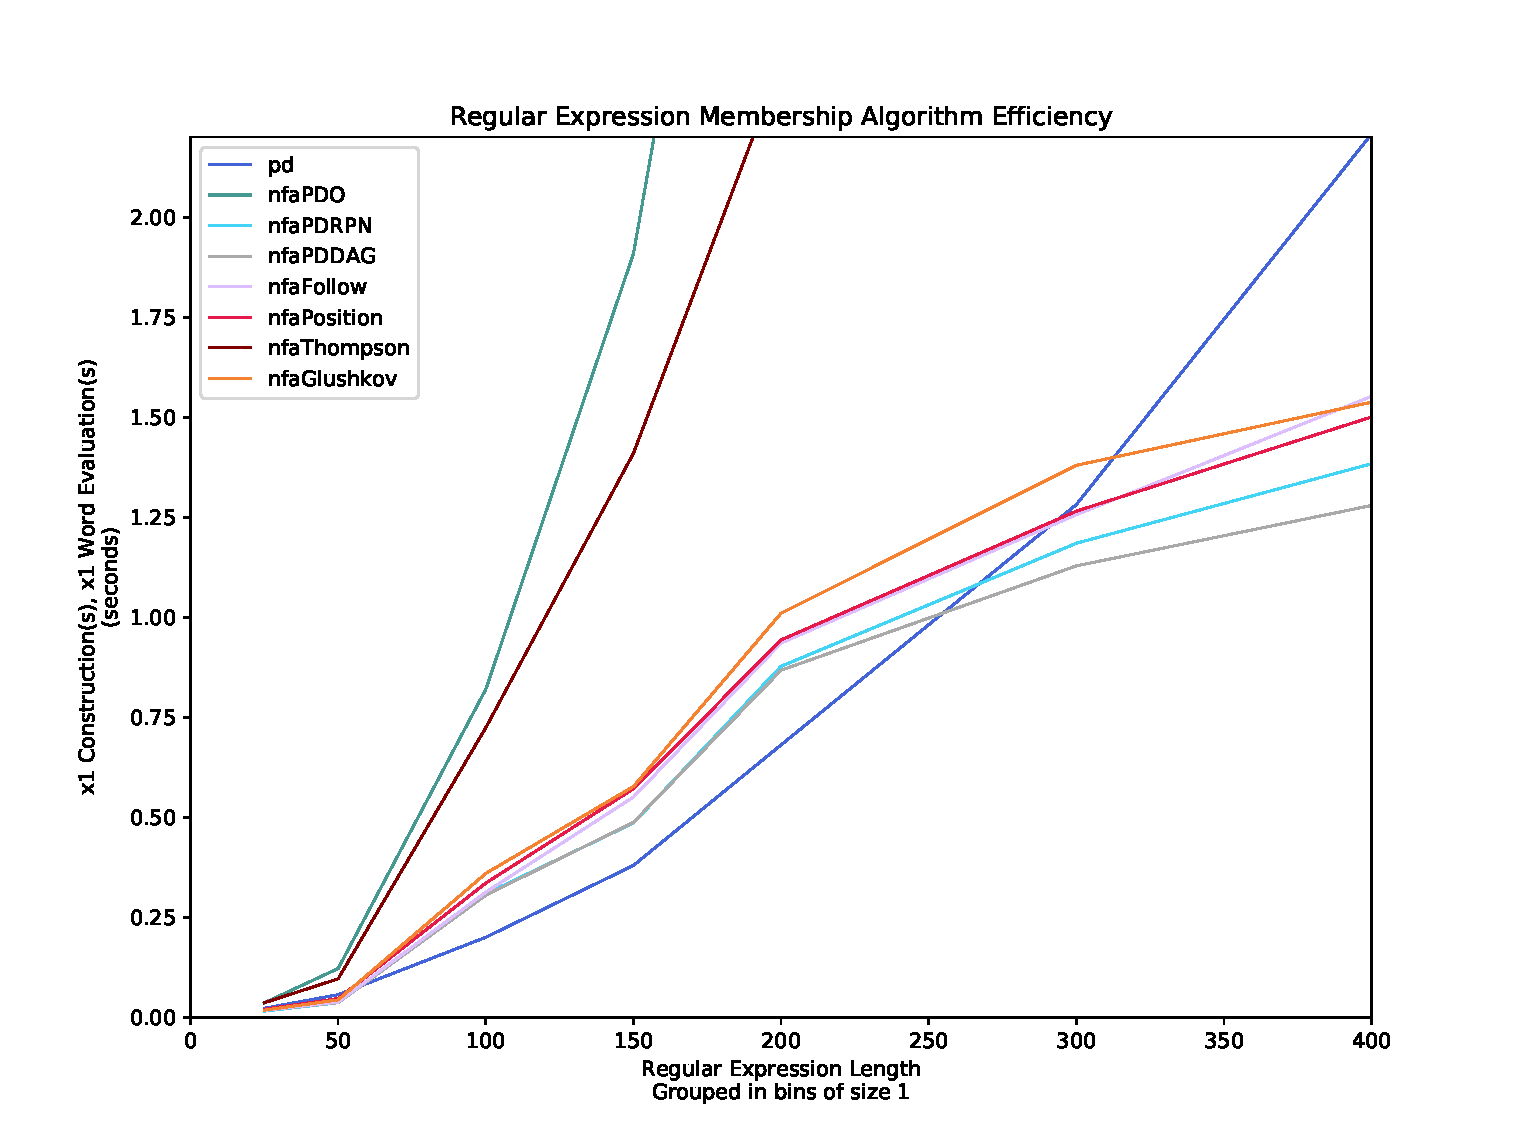
\includegraphics[width=0.75\linewidth]{fig/rand/1const1eval}
  \caption{Sum of construction time and one-word membership time for randomly generated regular expressions}
  \label{fig:rand/1const1eval}
\end{figure}

Figure \ref{fig:rand/1const1eval} combines Figures \ref{fig:rand/1construction} and \ref{fig:rand/1evaluation} to show how much time would be taken to construct the string into a Python class, and then evaluate membership of one word. The long length of input words makes determining word membership slow, so the construction cost is mostly negligible in comparison. The only significant difference from Figure \ref{fig:rand/1evaluation} is the nfaPDO construction makes this method the slowest, despite word membership on the partial derivative NFA being fast. The Thompson and nfaPDO methods are very slow, the partial derivative algorithm is competitively fast except at tree length 400, and then in increasing order: nfaPDDAG, nfaPDRPN, position, follow, and Glushkov.

\begin{figure}[H]
  \center
  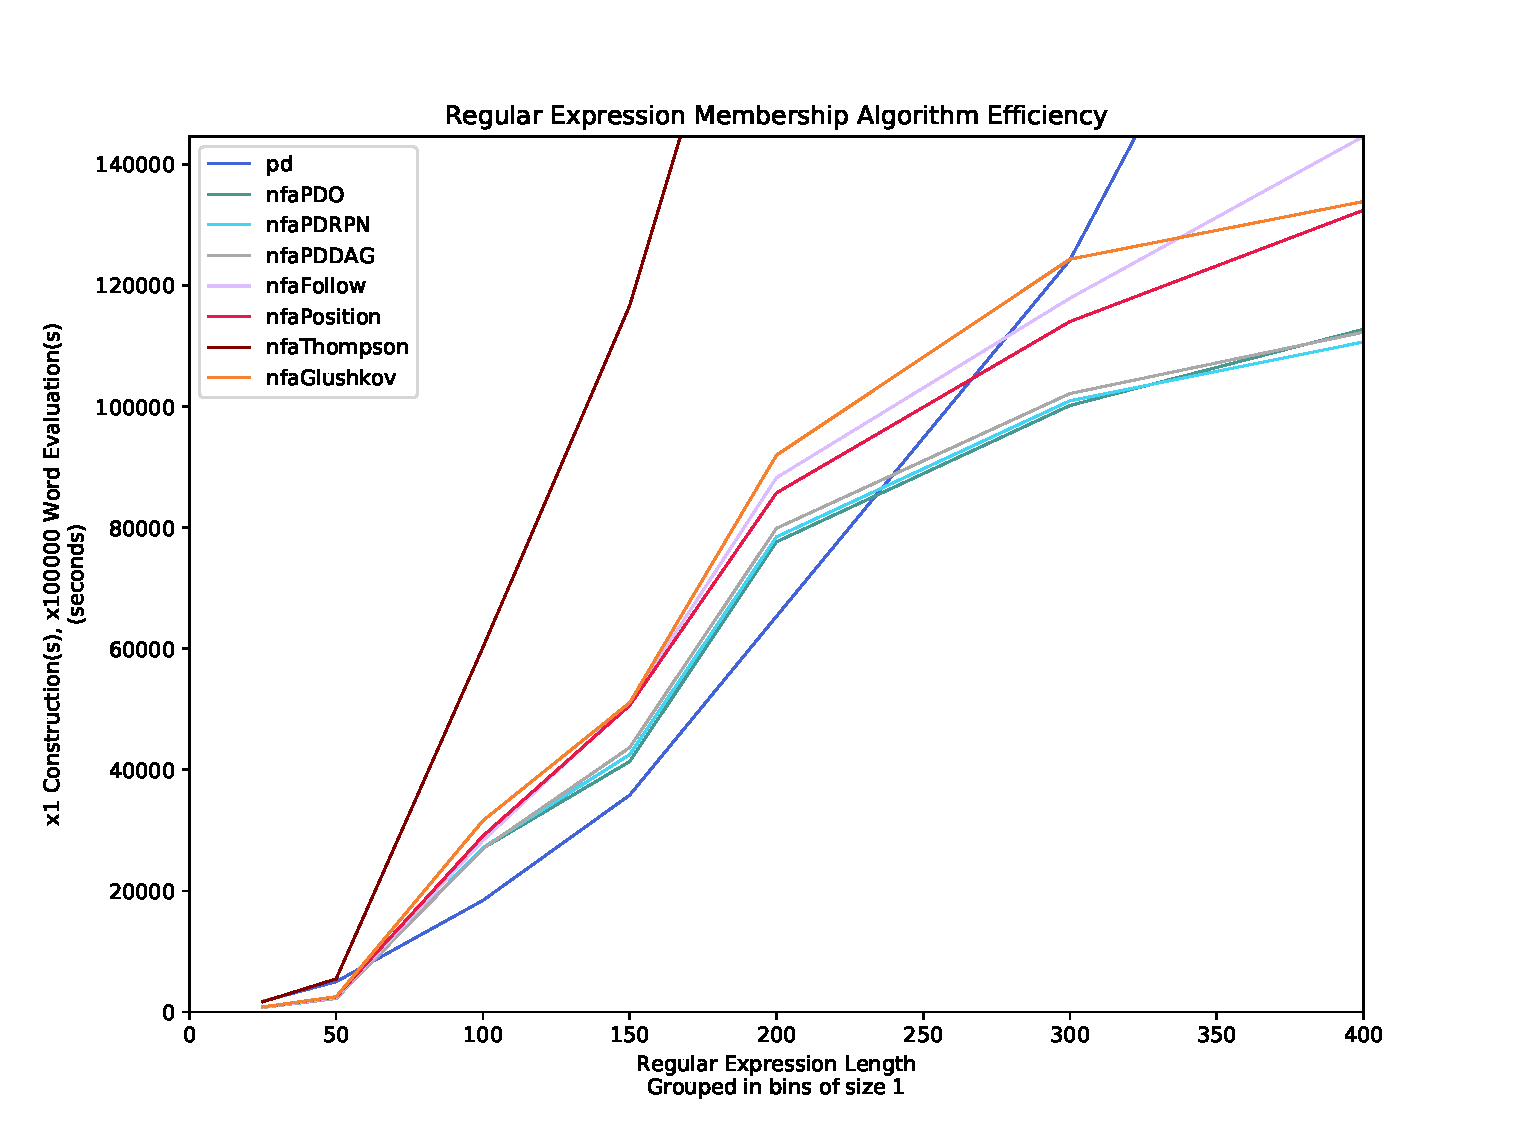
\includegraphics[width=0.75\linewidth]{fig/rand/1const10e6eval}
  \caption{Sum of construction time and 100,000 word membership time for randomly generated regular expressions}
  \label{fig:rand/1const10e6eval}
\end{figure}

There is little difference between Figure \ref{fig:rand/1const1eval} and Figure \ref{fig:rand/1const10e6eval}, only that the nfaPDO algorithm is once again competitive because the one-time construction cost is negligible in comparison to the membership cost.










  
  \chapter{Conclusions}
  \label{ch:Conclusions}
  Both theoretically and through experimentation we have shown the benefits and pitfalls of the common backtracking algorithm for word membership. This algorithm is suitable for applications that absolutely require non-regular language operations such as backreferences, or when developers create regular expressions that are robust against excessive backtracking. However, this method occasionally takes extreme membership time (e.g., randomly generated regular expressions, or pathologically chosen expressions designed to hog system resources). Any regular expression library using the backtracking algorithm should do so cautiously, and warn their users to avoid writing regular expressions vulnerable to a lot of backtracking.

Library and language developers cannot guarantee their users will write robust regular expressions, and many programmers consider regular expressions a ``black box'' of abstraction. If non-regular language operations are non-essential, or a regular expression contains only regular operations, then a more traditional theoretical algorithm is warranted. These algorithms provide polynomial worst case membership matching on any regular expression or input word combination, and therefore is safer for developers who use regular expressions without understanding their underlying implementation. Algorithms that first compute an NFA, and then run membership on that NFA should avoid NFA constructions involving empty transitions (like the Thompson construction) since they delay word matching. Instead, these sequential NFA constructions should be considered by increasing construction cost: follow, position, Glushkov, and PDDAG. The PDDAG NFA is slower to construct than the follow NFA, but is smaller on average and therefore results in faster membership times than any other considered NFA. Finally, non-NFA partial derivative membership could be fast if tree identification is done efficiently, and when binary concatenations grow right instead of left. Further research should compare these results when expanding concatenation trees right instead of left (Figure \ref{fig:left vs right expansion}), or potentially when building more complete trees. The trade-offs between parsing speed in Lark \cite{lark} and various regular expression/NFA algorithms would be an interesting investigation. Predominantly, evaluating membership using pure partial derivatives is expected to be much faster when expanding repetitions right.

Additionally, the speed of these tests proved to be a significant issue. They were executed over the span of months, and we still did not have time to finish all benchmarks. Using smaller test-sets of input words would speed up the overall time, and the pairwise generation algorithm \cite{pairgen} would have greatly benefited from a non-binary concatenation. However, the pairwise generation algorithm would still create long accepting words for deeply nested stars, and this needs to be addressed. Running these experiments in C++, Java, Rust, or even JavaScript would decrease execution time by up to hundreds of times; Python makes code quick to write, but \emph{ridiculously} slow to run.

If finding a database of perfectly accurate practical regular expressions was important to future researchers, they may approach the problem using grep.app to find relevant GitHub source files. But a significant improvement would be to parse the entire source file, and then traverse the parse tree to find regular expressions directly.

The source files and database results of this research are publicly available on GitHub, at \url{https://github.com/just1ngray/SMUHon-Practical-RE-Membership-Algs}.














  
  \printbibliography[title=References]
  
\end{document}




















